\documentclass[a4paper,parskip=half,BCOR=8mm,DIV=calc,12pt]{scrbook}

%\usepackage{german}
\usepackage[T3,T1]{fontenc}
\usepackage[utf8]{inputenc}
\usepackage{amsmath}
\usepackage{amsfonts}
\usepackage{amssymb}
\usepackage{mathtools}
\usepackage{stmaryrd}
\usepackage{faktor}
\usepackage{nicefrac}
\usepackage{listings}
\usepackage{enumerate}
\usepackage{dsfont}
\usepackage{remreset}
\usepackage{booktabs}
\usepackage{lettrine}
%\usepackage{txfonts}
\usepackage{varioref}
\usepackage{multirow}
\usepackage{rotating}
\usepackage{cancel}
\usepackage[pdfauthor={Joachim Breitner}]{hyperref}
\usepackage[capitalise]{cleveref}
\usepackage{tikz}
\usetikzlibrary{arrows,shapes}
% \usetikzlibrary{automata}
% \usetikzlibrary{decorations}
% \usetikzlibrary{snakes}
\usepackage{microtype}
\usepackage{framed}
\usepackage{caption}
\usepackage[normalem]{ulem}

%\usepackage{tipa} Causes warnings with \iff
\DeclareTextSymbol\textlambda{T3}{171}           % Lambda
\DeclareTextSymbolDefault\textlambda{T3}


\usepackage{isabelle,isabellesym}
\isabellestyle{it}

\newcommand{\isasymbinit}{\isamath{b_0}}
\newcommand{\isasymabinit}{\isamath{\widehat{b_0}}}
\newcommand{\isasymPR}{\isamath{\mathcal{PR}}}
\newcommand{\isasymaPR}{\isamath{\widehat{\mathcal{PR}}}}
\newcommand{\isasymanb}{\isamath{\widehat{{nb}}}}
\newcommand{\isasymaA}{\isamath{\widehat{\mathcal{A}}}}
\newcommand{\isasymaF}{\isamath{\widehat{\mathcal{F}}}}
\newcommand{\isasymaC}{\isamath{\widehat{\mathcal{C}}}}
% Types
\newcommand{\isasymabenv}{\isamath{\widehat{{benv}}}}
\newcommand{\isasymavenv}{\isamath{\widehat{{venv}}}}
\newcommand{\isasymaclosure}{\isamath{\widehat{{closure}}}}
\newcommand{\isasymaproc}{\isamath{\widehat{{proc}}}}
\newcommand{\isasymad}{\isamath{\widehat{{d}}}}
\newcommand{\isasymafstate}{\isamath{\widehat{{fstate}}}}
\newcommand{\isasymacstate}{\isamath{\widehat{{cstate}}}}
\newcommand{\isasymaccache}{\isamath{\widehat{{ccache}}}}
\newcommand{\isasymaans}{\isamath{\widehat{{ans}}}}

\newcommand{\isactrlps}[1]{{\uline #1}}


\usepackage[numbers,square]{natbib}
\bibliographystyle{amsplain}

% URLstyle
\urlstyle{rm}

% for \autoref
\newcommand{\examplename}{Example}
\newcommand{\lemmaname}{Lemma}
\newcommand{\remarkname}{Remark}
\newcommand{\corollaryname}{Corollary}
\newcommand{\definitionname}{Definition}
\newcommand{\algocflinename}{Algorithm}
\newcommand{\AlgoLineautorefname}{line}
\renewcommand{\chapterautorefname}{Chapter}
\renewcommand{\sectionautorefname}{Section}
\renewcommand{\subsectionautorefname}{Section}

% for \cref
\crefname{algocf}{Algorithm}{Algorithms}
\crefname{figure}{Figure}{Figure}

% vref settings
\vrefwarning
\def\reftextfaceafter {\unskip}%
\def\reftextfacebefore{\unskip}%
\def\reftextafter     {on the \reftextvario{following}{next} page}%
\def\reftextbefore    {on the \reftextvario{preceding}{previous} page}%
\def\reftextcurrent   {\unskip}%

% titlesec
\usepackage{titlesec}
\titleformat{\chapter}[display]
	{\sectfont\Large\filcenter}
	{\titlerule%[1pt]%
	 \vspace{1pt}%
	 \titlerule%
	 %\vspace{.4pc}%
	 \LARGE\MakeUppercase{\chaptertitlename} \thechapter}
	{1pc}
	{\titlerule
	 \vspace{1pc}%
	 \Huge}
% \titleformat{\chapter}[display]
% 	{\sectfont\Large}
% 	{%\titlerule%[1pt]%
% 	 %\vspace{1pt}%
% 	 %\titlerule%
% 	 %\vspace{.4pc}%
% 	 \LARGE{\chaptertitlename} \thechapter}
% 	{1pc}
% 	{%\titlerule
% 	 %\vspace{1pc}%
% 	 \sectfont%
% 	 \Huge}

%\pagestyle{headings}

\usepackage{mathpazo}

% Palatino: 5% mehr Zeilendurchschuss (laut KOMA-skript)
\linespread{1.05}

% Satzspiegel neu berechen
\recalctypearea


% Figures unabhängig vom Kapitel zählen
\makeatletter
\@removefromreset{figure}{chapter}
\renewcommand{\thefigure}{\arabic{figure}}
\@removefromreset{table}{chapter}
\renewcommand{\thetable}{\arabic{table}}
\makeatother

% Disable single lines at the start of a paragraph (Schusterjungen)
\clubpenalty = 10000
%
% Disable single lines at the end of a paragraph (Hurenkinder)
\widowpenalty = 10000 \displaywidowpenalty = 10000

% Remove skip between caption and figure.
\captionsetup[figure]{skip=0pt}

% listings
\lstset{language=Haskell
	,flexiblecolumns=True
	,columns=fullflexible
	,texcl=true
	,escapechar=!
	,basicstyle=\sffamily
	,stringstyle=\itshape
	,showstringspaces=false
	,literate={->}{$\to\,\,$}2 {→}{$\to\,\,$}2 {\\}{\textlambda}1
	}

% inputenc stuff
\DeclareUnicodeCharacter{03BB}{\textlambda}

% FrameSep default
\setlength{\FrameSep}{2pt}

% Float placement
%\renewcommand{\topfraction}{.95}
%\renewcommand{\bottomfraction}{.7}
%\renewcommand{\textfraction}{.05}
\renewcommand{\floatpagefraction}{.60}
%\renewcommand{\dbltopfraction}{.66}
%\renewcommand{\dblfloatpagefraction}{.66}
\setcounter{topnumber}{1}
\setcounter{bottomnumber}{1}


\newcommand{\C}{\mathcal C}
\newcommand{\F}{\mathcal F}
\newcommand{\PR}{\mathcal {PR}}
\newcommand{\A}{\mathcal A}


\newcommand{\aC}{\widehat{\mathcal C}}
\newcommand{\aF}{\widehat{\mathcal F}}
\newcommand{\aPR}{\widehat{\mathcal {PR}}}
\newcommand{\aA}{\widehat{\mathcal A}}

\newcommand{\N}{\mathds N}
\newcommand{\da}{\coloneqq}
\newcommand{\id}{\text{id}}
\newcommand{\fix}{\text{fix}}

\hyphenation{Karls-ruhe}

\author{Joachim Breitner}
\title{Control Flow in Functional Languages}
\subtitle{Formally taming lambdas}

\begin{document}
%\KOMAoptions{twoside=false}
\begin{titlepage}
\centering
\makeatletter
\textsc{\Large{Karlsruher Institut für Technologie}}\\
\vspace{.5em}
\textsc{\Large{Fakultät für Informatik}} \\
\vspace{4em}
{\Large \@author} \\
\vspace{2em}
{\large Student Research Project}\\
\vspace{2.5em}
{\sectfont\LARGE \@title }\\
\vspace{2em}
{\sectfont\Large \@subtitle }\\
% \vfill
% \begin{tikzpicture}[auto]
% \end{tikzpicture} \\
\vfill
Supervisors: \\
Prof. Dr. Gregor Snelting \\
Andreas Lochbihler \\
\vspace{2em}
{\@date }
\makeatother
\end{titlepage}
%\KOMAoptions{twoside=true}


\chapter*{Abstract}

\lettrine I{n} his dissertation\cite{Shivers}, Olin Shivers introduces a concept of control flow graphs for functional languages, provides an algorithm to statically derive a safe approximation of the control flow graph and proves this algorithm correct. In this student research project, Shivers’ algorithms and proofs are formalized using the theorem prover system Isabelle.


\tableofcontents
\enlargethispage{2em}
%\listoffigures

\chapter{Introduction}

\lettrine C{ontrol} Flow Analysis plays an important role in compiler construction as well as in security analysis. Having the latter case in mind, Daniel Wasserrab provides a formally verified slicing framework acting on an abstract and language-independent control flow graph in his dissertation\citep{wasserrab}. This framework has been instantiated for programs written in either a simple toy imperative language  or the Java-like language Jinja\citep{jinja}.

All these programming languages are imperative. Therefore, we are interested in its applicability to functional languages. This requires a notion of a control flow graph for functional programs. In 1991, Olin Shivers defined such a control flow graph and developed a static analysis algorithm to calculate it. Later research on functional control flow is often based on his definition.

To be able to connect to Wasserrab’s framework, the definitions and algorithms of Shivers need to be formalized in the theorem prover system Isabelle. This is the main goal of this project, although we treat the actual connection only theoretically.

This document starts with a concise overview of Shivers’ approach in \cref{chapshivers}. Then we explain the prototype in Haskell (\cref{chaphaskell}) as well as the formalization in Isabelle (\cref{chapisabelle}), stating where it differs from the original. We motivate some of the more interesting choices in the formalization, such as the use of \isa{HOLCF}. Some lemmas took several failed or unsatisfying attempts, which we do not hush up. We took special care to make the appearance of the documents generated by Isabelle as similar to the original as possible. \cref{seclayout} presents the tricks used to that end. \cref{chapslicing} explains the how these results could be connected to Wasserrab’s framework.

A total of 3625 lines of Isabelle code (including comments) and 890 lines of Haskell code (including 199 lines of commentary) were written.


% \vfill
% \lettrine[nindent=1ex]I{} owe sincere thanks to Dr.\ Gabriela Schmithüsen, under whose guidance this thesis was created. She was always generous with time, advice, regular proof-reading, ideas and inspiration.
% 
% Moreover, I wish to thank Mareike Schmidtobreick and Pascal Maillard for proof-reading the final work.

\chapter{Taming Lambdas}
\label{chapshivers}

\lettrine F{unctional} languages, i.e.\ programming languages that treat computations as first class citizens, are harder to tackle by control flow analysis than imperative languages. For the latter, a function call names the function that will be called and a static analysis can easily trace the control flow at that point. In functional languages, the callee can be a variable which, in turn, can stand for any computation that was stored somewhere else in the program.

Additionally, such a stored computation is a \textit{closure}, i.e.\ it remembers the variable  assignments from the time the closure was created. Therefore, a variable can have more than one current value at any given point in the program execution, where different closures see different values. This is an additional issue when trying to statically make statements about a functional program’s control flow.

Shivers approaches this problem in his 1991 Ph.D.\ thesis, subtitled “taming lambdas”. He defines an exemplary functional language in \textit{continuation-passing style} (CPS). CPS means that the return value of functions is not actually returned, but rather passed on to a continuation function, which is provided as an argument. Consider for example the following code :
\begin{lstlisting}[language=Haskell]
main = print ((x + y) * (z - w))
\end{lstlisting}
In continuation-passing style, the each of the operations \lstinline!+!, \lstinline!*!, \lstinline!-! and \lstinline!print! takes a continuation argument, and the \lstinline!main! function is being passed a top-level continuation: 
\begin{lstlisting}[language=Haskell]
main c = + x y (\xy. - z w (\zw. * xy zw (\prod. print prod c)))
\end{lstlisting}

\section{Syntax}

\begin{figure}
\begin{framed}
\begin{align*}
\text{PR} &\Coloneqq \text{LAM} \\
\text{LAM} &\Coloneqq (\lambda\ (v_1\ldots v_n)\ c) && [v_i\in \text{VAR},\, c\in\text{CALL}] \\
\text{CALL} &\Coloneqq (f\ a_1 \ldots a_n) && [f\in \text{FUN},\, a_i\in\text{ARG}] \\
&\phantom{\strut\Coloneqq\strut} (\text{\texttt{letrec}}\ ((f_1\ l_1)\ldots)\ c) && [f_i\in \text{VAR},\,l_i\in\text{LAM},\,c\in\text{CALL}] \\
\text{FUN} &\Coloneqq \text{LAM} + \text{REF} + \text{PRIM} \\
\text{ARG} &\Coloneqq \text{LAM} + \text{REF} + \text{CONST} \\
\text{REF} &\Coloneqq \text{VAR} \\
\text{VAR} &\Coloneqq \{\text{\texttt{x},\texttt{y},\texttt{foo},}\ldots\} \\
\text{CONST} &\Coloneqq \{\text{\texttt{3},\texttt{\#f},}\ldots\} \\
\text{PRIM} &\Coloneqq \{\text{\texttt{+},\texttt{if},\texttt{test-integer},}\ldots\} \\
\text{LAB} &\Coloneqq \{l_i,r_i,c_i,\ldots\} %ic_p^j\ldots\}
\end{align*}
\end{framed}
\caption{CPS syntax}
\label{fig:syntax}
\end{figure}

The syntax of Shivers’ toy functional programming language is given in \vref{fig:syntax}. A program (PR) is a lambda expression. A lambda expression (LAM) abstracts a call. Calls (CALL) either call a function with the given argument list or bind lambdas to names. Such calls are named \lstinline-letrec- because the bound lambdas may refer to each other in a possibly mutually recursive fashion, making the language Turing-complete.

Function values (FUN) can be lambda expressions, references to variables or primitive operations, while in argument positions (ARG), primitive operations are disallowed and constant expressions are allowed. References to variables (REF) name the referenced variable. There is a set of variable names (VAR). Constants (CONST) are either integers or \#f for a false value. A number of primitive operations (PRIM) are defined. Shivers treats mutable references and adds corresponding primitive operations in later chapters of his dissertation. We omit this and concentrate on the primitive operations \texttt+ and \texttt{if}.

Although not given explicitly, every lambda, call, constant, variable reference and primitive operation is tagged with a unique label from the set LAB. These can be thought of as positions in the program source – for our purpose they are just an abstract set.  Additional \textit{internal labels} are added to this set for primitive operations, representing the internal call sites. For example the \texttt{if} primitive operation is being passed two continuation that might be called, one for the true case and one for the false case. Therefore, two internal labels are associated with this primitive operation. Also we assume that programs are alphatised, i.e.\ each variable name $v$ is bound at exactly one position, whose label is given by $\text{\textit{binder}}\ v$.

\section{Standard Semantics}
\begin{figure}
\setlength{\FrameSep}{0pt}
\begin{framed}
\begin{align*}
\text{Bas} &= \mathds Z + \{\text{false}\} 
						& \mathllap{\PR} &\colon \text{PR} \rightharpoonup \text{Ans} \\
\text{Clo} &= \text{LAM} \times \text{BEnv} 
						& \A &\colon \text{ARG}\cup\text{FUN} \to \text{BEnv} \to \text{VEnv} \to \text{D} \\
\text{Proc} &= \text{Clo} + \text{PRIM} + \{\text{\textit{stop}}\} 
						& \C &\colon \text{CALL}\to \text{BEnv} \to \text{VEnv} \to \text{CN} \rightharpoonup \text{Ans} \\
\text{D} &= \text{Bas} + \text{Proc}
						& \F &\colon \text{Proc}\to \text{D}^* \to \text{VEnv} \to \text{CN} \rightharpoonup \text{Ans} \\
\text{CN} &= \text{\textit{(contours)}} \\
\text{BEnv} &= \text{LAB} \rightharpoonup \text{CN} \\
\text{VEnv} &= (\text{VAR}\times\text{CN}) \rightharpoonup \text{D}\\
\text{Ans} &= (\text D + \{\text{\textit{error}}\})_\bot
\end{align*}
\end{framed}
\caption{CPS semantics domains}
\label{fig:semdoms}
\end{figure}


Shivers gives a denotational semantics for the above language, that is a partial function $\PR$ from the set of programs to the set of integers with an additional element indicating run-time errors (Ans). Following the structure of the syntax tree, he defines functions $\C$, $\F$ and $\A$ that evaluate call expressions, apply arguments to procedures and evaluate argument expressions, respectively. Their domains and ranges are given in \vref{fig:semdoms}. The rather lengthy equations of their definitions are omitted here.

Semantic values (D) can either be basic values (Bas) which consist of the integers plus the value representing false, or a procedure. Procedures (Proc) again are either a closure (Clo), which is a lambda expression bundled with a context, a primitive operation or \textit{stop}.

The special value \textit{stop} is the continuation initially passed to the program. When this is eventually called, either in a CALL expression or as the continuation of a primitive operation, the evaluation comes to a halt and the argument to \textit{stop} is the result of the evaluation. If a run-time error occurs (wrong number of arguments, callee not a procedure, undefined variable lookup), \textit{error} is returned.

The semantics functions are partial functions, indicated by the harpoon instead of the arrow and by the $\bot$ annotation of the set Ans of answer values. Functional programs are Turing-complete and therefore possibly non-terminating. For such programs, the semantics is defined to return $\bot$.

The evaluation context needs to be passed along the semantics functions and closure values need to encapsulate the context at the time the lambda expression is evaluated to a closure. The context information is separated into two maps here: The global \textit{variable environment} (VEnv) and the lexical \textit{contour environment} (or binding environment, BEnv, in the following usually denoted by $\beta$). The variable environment can store multiple values for each variable name. These are differentiated by a \textit{contour number} from the set CN. These can be thought of time stamps which are increased in every evaluation step. When a variable is bound to a new value, it is stored in the variable environment with the current contour number. The contour environment tells for each binding position (lambda or \texttt{letrec} expression) which contour counter is to be used when looking up a variable bound there. By storing the contour environment within a closure and using it when evaluating the call inside the closure, the correct value for each variable binding is accessed.

The set CN of contours is not given explicitly here. Instead, we will treat it abstractly and only state the properties we expect from this set: There needs to be an initial contour $b_0$ and a function $nb \colon \text{CN} \to \text{CN}$ which generates new contours. The set of contours is partially ordered and if $b$ is greater or equal than all allocated contours, then $nb\ b$ is strictly greater than all allocated contours. It is easy to see that the natural numbers with $b_0 = 0$ and $nb\ b = \text{Suc}\ b$ fulfill the requirements, but in the later proofs it will be convenient to choose other sets carrying more information. 

\section{Exact nonstandard semantics}

\begin{figure}
\begin{framed}
\begin{align*}
\C\ (c:(f\ a_1\ldots a_n))\ \beta\ ve\ b &= 
\begin{cases}
[], & f' \notin \text{Proc} \\
(\F\ f'\ av\ ve\ b' )[(c,\beta) \mapsto f'], &\text{otherwise}
\end{cases}\\
&\phantom{\strut=\strut}\text{where } 
\begin{aligned}[t]
f' &= \A\ f\ \beta\ ve \\
av_i &= \A\ a_i\ \beta\ ve\\
b' &= nb\ b
\end{aligned}
\end{align*}
\vspace{-1em}
\end{framed}
\caption{The exact nonstandard semantics for a call expression}
\label{fig:callsem}
\end{figure}

At the moment we are not so much interested in the value a program returns but rather the calls that occur while evaluating the program. To that end we alter the standard semantics introduced in the previous section to calculate the \textit{call cache}. This is a partial map from call-site/contour-environment pairs to procedures. We therefore modify the domains of the semantics in \vref{fig:semdoms} as follows:
\begin{align*}
\text{CCache} &= (\text{LAB}\times\text{BEnv}) \rightharpoonup \text{Proc}\\
\text{Ans} &= \text{CCache}
\end{align*}

The semantics function definitions are extended to record the calls as they happen. \vref{fig:callsem} shows exemplary the equation of $\C$ for a call expression $(f\ a_1\ldots a_n)$ with label~$c$. If the syntactic value $f$ is evaluated to a procedure $f'\in \text{Proc}$, evaluation continues by applying $\F$ to $f'$ and the arguments. This returns a call cache, which is amended by the entry $(c,\beta) \mapsto f'$ to reflect the current call before the updated call cache is returned by~$C$.

This semantics evaluates the program in full, just like the standard semantics, and is therefore unsuitable to be used in a static analysis. Nevertheless it is the theoretic ideal that a statically calculated call cache will be compared against.

\section{Abstract nonstandard semantics}

Shivers then proceeds to define a nonstandard semantics that can be calculated statically. The trade off is that the call cache obtained now is just an approximation to the exact call cache, i.e.\ any observed call in the exact call cache will be in the abstract call cache, but the converse does not need to hold.

\begin{figure}
\setlength{\FrameSep}{0pt}
\begin{framed}
\begin{align*}
\widehat{\text{Clo}} &= \text{LAM} \times \widehat{\text{BEnv}}
& \widehat{\text{BEnv}} &= \text{LAB} \rightharpoonup \widehat{\text{CN}} \\
\widehat{\text{Proc}} &= \widehat{\text{Clo}} + \text{PRIM} + \{\text{\textit{stop}}\} 
& \widehat{\text{VEnv}} &= (\text{VAR}\times \widehat{\text{CN}}) \rightharpoonup \widehat{\text{D}} \\
\widehat{\text{D}} &= \mathcal P(\widehat{\text{Proc}})
& \widehat{\text{CCache}} &= (\text{LAB} \times \widehat{\text{BEnv}}) \to \widehat{\text{D}} \\
\widehat{\text{CN}} &= \text{\textit{(contours, finite)}} 
& \widehat{\text{Ans}} &= \widehat{\text{CCache}}
\end{align*}
\begin{align*}
\aPR &\colon \text{PR} \rightharpoonup \widehat{\text{Ans}} \\
\aA &\colon \text{ARG}\cup\text{FUN} \to \widehat{\text{BEnv}} \to \widehat{\text{VEnv}} \to \widehat{\text{D}} \\
\aC &\colon \text{CALL}\to \widehat{\text{BEnv}} \to \widehat{\text{VEnv}} \to \widehat{\text{CN}} \rightharpoonup \widehat{\text{Ans}} \\
\aF &\colon \widehat{\text{Proc}}\to \widehat{\text{D}}^* \to \widehat{\text{VEnv}} \to \widehat{\text{CN}} \rightharpoonup \widehat{\text{Ans}}
\end{align*}
\end{framed}
\caption{Abstract nonstandard semantics domains}
\label{fig:abssemdoms}
\end{figure}

\vref{fig:abssemdoms} gives the domains of the abstract semantics functions. The abstract semantics $\aPR$ will run the program no longer in full detail. It will not keep track of actual values computed and conditional branches taken. Instead, it assumes that every branch of an \texttt{if} statement is possibly taken. Semantic values are now sets of possible procedures. This can be seen in \vref{fig:ifsem}, which contains both the exact and the abstract nonstandard semantics definitions for an conditional expression. The continuations respectively, in the abstract case, the sets of possible continuations are passed as the arguments $c_0$ and~$c_1$.

\begin{figure}
\begin{framed}
\begin{align*}
\F\ \text{\texttt{if}}\ [v,c_0, c_1]\  ve\ b &=
\begin{cases}
[], \text{ if } c_0 \notin \text{Proc} \text{ or } c_1 \notin \text{Proc} \\
\{ (ip_0,\beta) \mapsto c_0 \} \cup \F\ c_0\ []\ ve\ (nb\ b),\text{ if } v \ne 0 \\
\{ (ip_1,\beta) \mapsto c_1 \} \cup \F\ c_1\ []\ ve\ (nb\ b),\text{ if } v = 0 
\end{cases}\\
&\phantom{\strut=}\text{where } \beta = \{ p \mapsto b \}
\end{align*}
\begin{align*}
\aF\ \text{\texttt{if}}\ [v,c_0, c_1]\  ve\ b &=
\phantom{\cup}\bigcup_{f\in c_0} \aF\ f\ []\ ve\ (\widehat{nb}\ b\ ip_0)\\
&\phantom{\strut=} \cup \bigcup_{f\in c_0} \aF\ f\ []\ ve\ (\widehat{nb}\ b\ ip_1)\\
&\phantom{\strut=} \cup \{ (ip_0, \beta) \mapsto c_0,\ (ip_1, \beta) \mapsto c_1\} \\
&\phantom{\strut=}\text{where } \beta = \{ p \mapsto b \}
\end{align*}
\vspace{-1em}
\end{framed}
\caption{Comparison of the nonstandard semantics for an conditional expression with label $p$ and internal labels $ip_0$ and $ip_1$ }
\label{fig:ifsem}
\end{figure}


After removing the plain values from our semantics domains, the remaining sets would all be finite – if $\widehat{\text{CN}}$ was finite. This is the main trick to obtain a computable abstract semantics. If $\widehat{\text{CN}}$ is finite, there are only finitely many possible closures, procedures, binding environment, variable environments and call caches, and our function becomes computable.

Naturally, there is a loss of information when replacing the infinite set of contour counters in the exact case by a finite set. Variable bindings that could otherwise be distinguished by their contour counter now fall together. Therefore, the abstract variable environment tracks sets of possible values for each variable/contour counter pair.

Again, the choice of the set $\widehat{\text{CN}}$ is not fixed. Possible choices include the singleton set, resulting in “0th-order Control Flow Analysis” (0CFA) or the set of lambdas representing the call site a lambda was called from, resulting in first-order Control Flow Analysis (1CFA). To be able to track this information, the function $\widehat{nb}$, used to generate new contour counters, takes such a label as an additional argument. It is ignored when performing 0CFA, and it is stored as the contour counter in 1CFA.

This generalizes to $k$CFA, where the last $k$ call sites are tracked by the abstract contour counter. The more information we store in the abstract contour counters, the more detailed our analysis will be, but also more expensive to calculate.

Because semantic values $\widehat{\text{D}}$ are now sets of procedures, when evaluating a call expression $(f\ a_1\ldots a_n)$, there is a set of possible procedures that $f$ can evaluate to, and $\aF$ will be called for each of them. The resulting call caches need to be joined by pointwise set union. Similarly, the continuations of primitive operations are sets of procedures, for all of which $\aF$ is called and the results are  joined, as seen in \cref{fig:ifsem}.

\section{Main results}

These main results about the semantics functions are stated and shown in Shivers’ dissertation:
\begin{enumerate}
\item The call cache returned by the exact semantics is indeed a partial map,
\item the abstract semantics approximates the exact semantics and
\item the abstract semantics is computable.
\end{enumerate}

But before starting to prove these results, Shivers establishes that the recursive definitions he gave for $\F$ and $\C$ (and by analogy, $\aF$ and $\aC$) are sound. He proceeds in the standard way of turning a recursive definitions $f = F f$ for a function $f\in X$, where $X$ is a function space with a chain-complete partial order, into a functional $F\colon X \to X$. $F$ is then shown to be continuous and therefore has a least fixed point, which serves as the definition of~$f$.
  

The need to show that the result of $\PR$ is a partial map arises from the fact that, for an easier proof of continuity, Shivers changes the answer domain to be
\[
\text{Ans} = \mathcal P( (\text{LAB}\times\text{BEnv}) \times \text{Proc}).
\]
The actual proof is only outlined in his dissertation.

In contrast, the proof that $\aPR$ safely approximates $\PR$ is given in full detail. For any of the types Proc, D, $\text{D}^*$, BEnv, VEnv, CN and CCache, he defines an abstraction function (written $|\cdot|$) from the exact type to the corresponding abstract type. He also defines partial orders on the abstract types (here written $\cdot \lessapprox \cdot$), expressing that one value is more specific than another value. The main result is then
\begin{quote}
\textbf{Theorem 6}: For any program $l$, call site label $c$ and binding environment $\beta$, we have
\[
|(\PR\ l)\ (c,\beta)| \lessapprox (\aPR\ l) (c,|\beta|).
\]
\end{quote}
The largest part of the proof is to show two similar statements relating $\F$ and $\aF$ resp. $\C$ and $\aC$. Because these are mutually recursive, both statements are shown in one big step.

The machinery to prove results about functions defined as fixed points is the fixed point induction: A predicate $P$ holds for the least fixed point of $F$ if the following three conditions are true:\label{fixedpointinduction}
\begin{itemize}
\item $P$ is an admissible predicate. This is closely related to continuity and states that if $P$ holds for each element of an infinite chain, it holds for the limit of the chain.
\item $P\ \bot$ holds.
\item If $P\ f$ is true, then $P\ (F\ f)$ is true.
\end{itemize}

\label{shiverscomputabilty}The computability result is not shown explicitly for $\aPR$, but rather for general recursive equations of the shape
\[
f\ x = g\ x \cup f\ (r\ x)
\]
where each function invocation makes a local contribution $g\ x$ to the result and then recurses with a new argument $r\ x$. Shivers shows that in that case, the least fixed point is given by
\[
f\ x = \bigcup_{i=0}^\infty g\ (r^i\ x).
\]
If additionally the argument space is finite, the infinite union is actually finite as well and the calculation is complete after a finite number of iterations.

The semantics functions $\aF$ and $\aC$ are nearly of this type, but they have a branch factor greater than one. Thus, for solution to an equations like
\[
f\ x = g\ x \cup \bigcup\{f\ x' \mid x' \in R\ x\}
\]
he introduces the \textit{powerset relative} of a function $h$ as $\uline h\ X\coloneqq \{h\ x \mid x\in X\}$ and transforms the above equation to 
\[
\uline f\ X = \uline g\ x \cup \uline f\ (\uline R\ Y)
\]
to be able to apply the previous result.

The required steps to apply this result to the mutually recursive definitions $\aF$ and $\aC$ are not explained in the dissertation.


\section{Example}
\label{examplesection}

\begin{figure}
\begin{framed}
\ttfamily
\footnotesize
\frenchspacing
\newcommand{\lab}[1]{\textsuperscript{\scriptsize\sffamily#1}}
\begin{tabbing}
(\=λ \=let rec = (\=λ \=then (\=λ .\=\ (\=+) p i (\=λ p'.\=\ (\=+) i -1 (\=λ i'.\=\ rec p' i' c')))\kill
(λ cont.\\
\>\lab{1}
\+\+\\
   let rec = (λ p i c'.\\
   \lab{2}\'\> \lab{3}
\+\+\\
                if i\\
\lab{4}\'\\
                then (λ . (+) p i (λ p'. (+) i -1 (λ i'. rec p' i' c')))\\
\lab{5} \> \lab{8} \> \lab{9} \> \lab{10} \> \lab{13} \> \lab{14} \> \lab{15} \> \lab{18} \>\lab{19} \\		
                else (λ . c' p))\\
\lab{6} \> \lab{24} \> \lab{25}
\-\-\\
   in rec 0 10 cont)\\
\ \ \lab{28}
\end{tabbing}
\vspace{-1em}
\end{framed}
\caption{CPS program calculating the sum of the first ten natural numbers}
\label{fig:examplecode}
\end{figure}


In \vref{fig:examplecode} lists a functional program in continuation-passing style, calculating the sum of the first ten natural numbers. Its code positions are subscripted by labels which are automatically assigned by the Haskell code presented in the following chapter. Lambda expressions have labels 1, 3, 8, 13, 18, and 24. Call expressions, where the label is placed below the space before the callee, are 2, 4, 9, 14, 19, 25 and 28. Labels 5 and 6 denote the two internal call sites of the conditional expression, while labels 10 and 15 denote the internal call sites of the two primops \texttt{(+)}.

A contour environment specifies for each binding position which binding, identified by a contour counter (in this section printed in italics to distinguish them from syntactical labels), is currently in place. The \texttt{let}-expression in the above code will store the lambda expression with label 3 in the variable environment, coupled with the contour environment
\[
\{ 1 \mapsto \textit 0,\ 2 \mapsto \textit 1 \}
\]
indicating that the variable \texttt{cont} should resolve to the value bound when the contour counter was \textit 0 and that \texttt{rec} should resolve to the value bound when the contour counter was \textit 1. The closure is called at label 28, which adds the following entry to the call cache calculated by the exact semantics
\[
(28,\ \{ 1 \mapsto \textit 0,\ 2 \mapsto \textit 1 \}) \mapsto (3,\ \{ 1 \mapsto \textit 0,\ 2 \mapsto \textit 1 \}).
\]
The lambda expression will store the values passed as arguments using the contour counter \textit 2 and passes the following, extended binding environment to call 4:
\[
\{ 1 \mapsto \textit 0,\ 2 \mapsto \textit 1, 3 \mapsto \textit 2\}.
\]

The next call of lambda 3, from position 19, is recorded in the exact call cache by
\begin{multline*}
(19,\ \{ 1\mapsto \textit 0,\ 2\mapsto \textit 2,\ 3\mapsto \textit 2,\ 8\mapsto \textit 4,\ 13\mapsto \textit 6,\ 18\mapsto \textit 8\}) \\ \mapsto (3,\ \{ 1 \mapsto \textit 0,\ 2 \mapsto \textit 1 \}).
\end{multline*}
Now, the arguments will be stored using the contour counter \textit 9 and call 4 is evaluated with a binding environment of 
\[
\{ 1 \mapsto \textit 0,\ 2 \mapsto \textit 1, 3 \mapsto \textit 9\},
\]
ensuring that the correct values of \texttt{p}, \texttt{i} and \texttt{c'} will be obtained when looking up these variables in the variable environment.

\begin{figure}
\begin{framed}
\vspace{-1em}
\begin{align*}
4 &\mapsto \{5\}
& 14 &\mapsto \{15\}\\
5 &\mapsto \{8\}
& 15 &\mapsto \{18\}\\
6 &\mapsto \{24\}
& 19 &\mapsto \{3\}\\
9 &\mapsto \{10\}
& 25 &\mapsto \{\text{\textit{Stop}}\}\\
10 &\mapsto \{13\}
& 28 &\mapsto \{3\}
\end{align*}
\end{framed}
\caption{0CFA-analysis of the example program}
\label{fig:examplecfa0}
\end{figure}

The complete exact call cache for this program contains 74 entries and we abstain from reproducing it here. The abstract call cache obtained using the 0CFA abstraction is given in \vref{fig:examplecfa0}. Since the contour environments carry no information in this case, they are omitted. Note that the label 5 on the right hand side of the edge $4 \mapsto \{5\}$ represents the whole if expression, not just the first branch.

Applying the 1CFA abstraction, we obtain the call cache in \vref{fig:examplecfa1}. The contour counter -1 represents the context “outside” the analyzed program.  The left hand sides of the entries, as well as closures on the right hand side, now carry their abstracted contour environment. In this example, it allows us to tell evaluations of the lambda expression 3 called from position 28 apart from those called from position 19. In our case, the gain is small as in either case we call the same procedures. % Primitive operations and \textit{Stop} on the right hand side do not carry a contour environment.

But consider the following lambda expression, which implements the function composition operator $\circ$ in continuation-passing style by evaluating \verb-g-, feeding the result to \verb-f- and passing evaluation on to the continuation \verb-c-:
\begin{center}
\ttfamily λ f g c . g (λ r. f r c)
\end{center}
If this function is used in two totally different contexts, a 0CFA analysis could not tell the two apart and would add return edges from $\circ$ to both of them. 1CFA would annotate those edges by the context that $\circ$ had been called in, and thus prevents mixing these different control flows.

But 1CFA cannot help if a commonly used function \verb-f- itself calls another function \verb-g- which then calls the continuation, as the context of \verb-g- is always within \verb-f- and \verb-f-’s context is lost. In that example, 2CFA would be required, and there is no general solution to this problem.
\enlargethispage{1em}

\begin{sidewaysfigure}
\begin{framed}
\vspace{-1em}
\small
\begin{align*}
(4,\{1\mapsto -1,\ 2\mapsto 2,\ 3\mapsto 19\}) &\mapsto \{5\}\\
(4,\{1\mapsto -1,\ 2\mapsto 2,\ 3\mapsto 28\}) &\mapsto \{5\}\\
(5,\{5\mapsto 4\}) &\mapsto \{(8,\{1 \mapsto -1,\ 2\mapsto 2,\ 3 \mapsto 28\})\}\\
(6,\{6\mapsto 4\}) &\mapsto \{(24,\{1 \mapsto -1,\ 2\mapsto 2,\ 3 \mapsto 28\})\}\\
(9,\{1\mapsto -1,\ 2\mapsto 2,\ 3\mapsto 19,\ 8\mapsto 5\}) &\mapsto \{10\}\\
(9,\{1\mapsto -1,\ 2\mapsto 2,\ 3\mapsto 28,\ 8\mapsto 5\}) &\mapsto \{10\}\\
(10,\{10\mapsto 9\}) &\mapsto \{(13, \{1 \mapsto -1,\ 2\mapsto 2,\ 3 \mapsto 28,\ 8\mapsto 5\})\}\\
(14,\{1\mapsto -1,\ 2\mapsto 2,\ 3\mapsto 19,\ 8\mapsto 5,\ 13\mapsto 10\}) &\mapsto \{15\}\\
(14,\{1\mapsto -1,\ 2\mapsto 2,\ 3\mapsto 28,\ 8\mapsto 5,\ 13\mapsto 10\}) &\mapsto \{15\}\\
(15,\{15\mapsto 14\}) &\mapsto \{(18,\{1\mapsto -1,\ 2\mapsto 2,\ 3\mapsto 28,\ 8\mapsto 5,\ 13\mapsto 10\})\}\\
(19,\{1\mapsto -1,\ 2\mapsto 2,\ 3\mapsto 19,\ 8\mapsto 5,\ 13\mapsto 10,\ 18\mapsto 15\}) &\mapsto \{(3, \{(8,\{1 \mapsto -1,\ 2\mapsto 2\})\}\\
(19,\{1\mapsto -1,\ 2\mapsto 2,\ 3\mapsto 28,\ 8\mapsto 5,\ 13\mapsto 10,\ 18\mapsto 15\}) &\mapsto \{(3, \{(8,\{1 \mapsto -1,\ 2\mapsto 2\})\}\\
(25,\{1\mapsto -1,\ 2\mapsto 2,\ 3\mapsto 19,\ 24\mapsto 6\}) &\mapsto \{\text{\textit{Stop}}\}\\
(25,\{1\mapsto -1,\ 2\mapsto 2,\ 3\mapsto 28,\ 24\mapsto 6\}) &\mapsto \{\text{\textit{Stop}}\}\\
(28,\{1\mapsto -1,\ 2\mapsto 2\}) &\mapsto \{(3,\{1 \mapsto -1,\ 2\mapsto 2)\})\}
\end{align*}
\end{framed}
\caption{1CFA-analysis of the example program}
\label{fig:examplecfa1}
\end{sidewaysfigure}


\chapter{The Haskell Prototype}
\label{chaphaskell}

\lettrine T{o} get a better understanding of the algorithms, we first implemented a prototype in Haskell. As the semantics are given in denotational style, they are easily translated into a functional program. The elements of the syntax definition of the CPS style language are directly turned into data type definitions, given in \vref{fig:haskelldatatypes}.

\begin{figure}
\begin{framed}
\begin{lstlisting}
type Prog = Lambda
newtype Label = Label Integer
data Var = Var Label String
data Lambda = Lambda Label [Var] Call
data Call = App Label Val [Val]
          | Let Label [(Var, Lambda)] Call
data Val = L Lambda
         | R Label Var
         | C Label Const
         | P Prim
type Const = Integer
data Prim = Plus Label
          | If Label Label 
\end{lstlisting}
\end{framed}
\caption{The Haskell representation of abstract syntax trees}
\label{fig:haskelldatatypes}
\end{figure}


At this point, we slightly deviate from the original: Shivers distinguishes the sets FUN and ARG as direct sums (cf.\ \vref{fig:syntax}) and later defines the function $\A$ on the union of FUN and ARG (cf.\ \vref{fig:semdoms}). This would be tedious and unwieldy to express in the Haskell type system, therefore we use one set VAL instead of FUN and ARG, which does not affect the algorithms in any notable way:
\begin{align*}
\text{VAL} &\Coloneqq \text{LAM} + \text{REF} + \text{PRIM} + \text{CONST}
\end{align*}
We also drop the special constant \texttt{\#f} representing false from the syntax and the corresponding value false from the set of semantic values, which are now just the integers. The \texttt{if} primitive operation considers zero as false and any other integer as true.

\section{Type system tricks}

As mentioned in the last chapter, most elements of the syntax carry a label. These labels need to be unique and every mention of a variable needs to carry the label of the variable’s binding position. To prevent the hypothetical user of the library from getting the labels wrong, we exploit the \textit{smart constructor} idiom.

\begin{figure}
\begin{framed}
\centering
\begin{lstlisting}
-- Returns the sum of the first 10 natural numbers            
ex3 :: Prog
ex3 = prog $ lambda ["cont"] $
        let_ [("rec", lambda ["p", "i", "c'"] $
                        app if_
                            [ "i"
                            , l $ lambda [] $
                                app plus ["p", "i",
                                    l $ lambda ["p'"] $
                                        app plus ["i", -1,
                                            l $ lambda ["i'"] $
                                                app "rec" [ "p'", "i'",  "c'" ]
                                            ]
                                    ]
                            , l $ lambda [] $
                                app "c'" ["p"]
                            ]
        )] $ app "rec" [0, 10, "cont"]
\end{lstlisting}
\end{framed}
\caption{Example code, defined using smart constructors}
\label{fig:sum10}
\end{figure}

A type alias marks not-fully-constructed syntax tree values and prevents their use in other functions.
\begin{lstlisting}
newtype Inv a = Inv { unsafeFinish :: a } deriving (Show, Eq)
\end{lstlisting}
The deconstructor \lstinline!unsafeFinish :: Inv a → a! is only to be used internally.

Now a value of type \lstinline-Inv Lambda- represents a lambda expression without correct labels. For each constructor there is a function (the smart constructor), taking the same arguments except the label, and building the unfinished value. We named it after the constructor it replaces, written lower case. Because \lstinline-let- and \lstinline-if- are keywords in Haskell, the corresponding smart constructors are called \lstinline-let_- and \lstinline-if_-. For example, the smart constructor for lambda expressions is defined as
\begin{lstlisting}
lambda :: [Inv Var] -> Inv Call -> Inv Lambda
lambda vs (Inv c) = Inv $ Lambda noProg (map unsafeFinish vs) c
\end{lstlisting}
where \lstinline!noProg! throws, if it were evaluated, an exception:
\begin{lstlisting}
noProg :: a
noProg = error "Smart constructors used without calling prog"
\end{lstlisting}


There is only one function for public consumption that removes the \lstinline-Inv--wrapper, with signature \lstinline!prog :: Inv Lambda -> Prog!. It uses a state monad to hand out unique labels and keeps track of variable bindings to correctly set the reference to the binding position. 

For additional convenience, we made the types \lstinline!Var!, \lstinline!Val! and \lstinline!Inv a! instances of the \lstinline!IsString! type class which allows the compiler, if the language extension \lstinline!OverloadedStrings! is enabled, to turn string literals into values of these kinds. Using the same trick, a \lstinline!Num!-instance for \lstinline!Val! allows to enter constants directly as literal numbers.

A simple example program, returning the result of the worldshaking calculation $1 + 1$, can now entered as
\begin{lstlisting}
ex2 :: Prog
ex2 = prog $ lambda ["cont"] $ 
        app plus [1, 1, "cont"]
\end{lstlisting}
instead of the much verbose
\begin{lstlisting}
ex2 :: Prog
ex2 = Lambda (Label 1) [Var (Label 1) "cont"] $
	App (Label 2) (P (Plus (Label 3))) [
		C (Label 4) 1,
	        C (Label 5) 1,
		R (Label 6) (Var (Label 1) "cont")].
\end{lstlisting}
A larger example is included in \vref{fig:sum10}, where the first ten natural numbers are added up.

%\section{Pretty Printing and Graphical Output}
\section{Pretty Printing}

Another feature of the Haskell prototype is pretty-printing of an abstract syntax tree. It uses the standard pretty printing library of Haskell \cite{pretty} and renders the above example to the string “\texttt{(λ\ cont.\ (+)\ 1\ 1\ cont)}”. \vref{fig:prettyprint} shows the pretty printed presentation of the program in \vref{fig:sum10}.

\begin{figure}
\centering
\begin{framed}
\footnotesize
\begin{verbatim}
(λ cont.
   let rec = (λ p i c'.
                if i
                then (λ . (+) p i (λ p'. (+) i -1 (λ i'. rec p' i' c')))
                else (λ . c' p))
   in rec 0 10 cont)
\end{verbatim}
\end{framed}
\caption{Pretty-printed output}
\label{fig:prettyprint}
\end{figure}

% After having pretty-printed the code, we wished we had a nice presentation of the call caches returned by the semantics functions. Recall that the call cache is a map from call sites, represented by labels, and binding environments to values. This can be turned into a map from labels to labels (hereby losing the context information) and thus arrows in the source code.
% 
% It turned out that the mapping from labels to coordinates in the source code is tricky to come by: The pretty printing library’s API offers no way of marking positions in the resulting string. An alternative would have been to re-implement the pretty printing library with this additional feature, but this would be out of scope for this project (even more than the graphical output). Instead we employed a hack abusing the wide range of characters that Unicode based strings provide: When pretty printing the code, labels (which are positive integers) are inserted as single characters with a code point of U+100000 plus the number of the label. These are in the Private Use Area of the Unicode specification.
% 
% \begin{figure}%
% \centering%
% \begin{framed}%
% 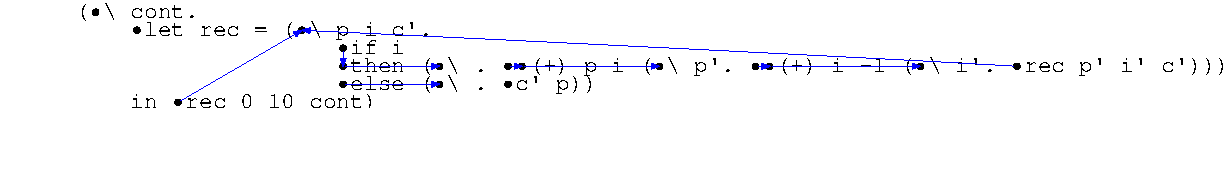
\includegraphics[width=\linewidth]{rendered-graph.pdf}%
% \end{framed}%
% \caption{The code annotated with the control cache}%
% \label{fig:ccgraph}%
% \end{figure}
% 
% After the pretty printer has laid out the code, we can gather the coordinates of all characters with code points larger or equal to U+100000 and replace them by a placeholder symbol (we chose $\bullet$). The pretty printed code is written to a PDF file using the HPDF library\cite{HPDF}, which is implemented in pure Haskell. This gives us maximal control over the positioning and allows us to render the document without padding.
% 
% To draw the arrows, we want to use the graphviz suite\cite{Graphviz} which includes several graph layout mechanisms. From the edges given by the control cache and the label coordinates from the pretty-printed code a graph description in the dot-format is generated and rendered to PDF using the \texttt{neato} command. The two PDF files are now mapped onto each other using \texttt{pdftk}\cite{pdftk}. If everything went right, the arrows will begin and end exactly at the character that replaced the label. A result is included in \vref{fig:ccgraph}.
% 
% This was just a quick experiment and serves as a proof-of-concept. Obviously, this presentation has its weakness, such as the reduced legibility of the code due to the arrows passing semi-transparently over the text.

Also, a conversion function is included that renders a program in the syntax used by Isabelle, to make it more convenient to obtain example programs within Isabelle.

\chapter{The Isabelle Formalization}
\label{chapisabelle}

\lettrine[lines=3]T{he} main mission of this student research project was to implement Shivers’ algorithms in the theorem prover Isabelle\citep{isabelle} and to prove his main results as introduced in \cref{chapshivers}. Shivers was already very rigorous and formal in his proofs, which helped a lot in the course of this project. The main hurdles to take were

\begin{itemize}
\item representing partial functions, such as the semantics functions, in Isabelle within the default logic HOL, which is a logic of total functions, and
\item obtaining the fact that the set of subterms of a program is finite.
\end{itemize}

\section{Structure}

\begin{figure}
\begin{framed}
\centering
%\includegraphics{sessionGraph.pdf}
\input{sessionGraph.tex}
\end{framed}
\caption{Isabelle theories and their dependencies}
\label{fig:sessionGraph}
\end{figure}

I separated the formalizations into several files (called theories in Isabelle-speak). Their dependencies are given in \vref{fig:sessionGraph}, where theories in rectangles contain definitions, boxed theories contain the main results and theories in rounded rectangles contain auxiliary definitions and lemmas. The definitional theories have directly corresponding counter-parts in the Haskell prototype. The following list gives a quick summary of their content.

\begin{description}
\setkomafont{descriptionlabel}{\itshape}
\setlength\parskip{0pt}
\item[CPSScheme] contains the definitions of the abstract syntax to represent the functional programs. The types (\vref{fig:isabelletypes}) are very similar to those in the Haskell prototype (\vref{fig:haskelldatatypes}).
\item[Eval] is an implementation of the standard semantics.
\item[ExCF] is an implementation of the exact nonstandard semantics.
\item[AbsCF] is an implementation of the abstract nonstandard semantics.
\vspace{1em}
\item[ExCFSV] proves that a call cache returned by the exact nonstandard semantics is indeed a partial map.
\item[AbsCFCorrect] proves that the abstract nonstandard semantics safely approximate the exact nonstandard semantics.
\item[Computability] contains Shivers’ general treatment of equations whose least solution is computable.
\item[AbsCFComp] applies the results from the previous theory to the abstract nonstandard semantics. This step was skipped by Shivers.
\vspace{1em}
\item[Utils] is a potpourri of various lemmas not specific to our project, some of which could very well be included in the default Isabelle library.
\item[HOLCFUtils] contains generic lemmas related to the use of \isa{HOLCF}, a domain theory extension to Isabelle.
\item[CPSUtils] defines sets of subterms for programs and proves their finiteness.
\item[FixTransform] transforms fixed point expressions defining two mutually recursive functions to fixed point expressions defining a single function.
\item[SetMap] contains functions and lemmas to work with set-valued maps.
\item[MapSets] defines sets of functions and sets of maps, and shows the finiteness of such maps, if their domains and ranges are finite.
\end{description}

\begin{figure}
\begin{framed}
%
\begin{isabellebody}%
\def\isabellecontext{CPSScheme}%
%
\isamarkuptrue%
\isacommand{types}\isamarkupfalse%
\ label\ {\isacharequal}\ nat\isanewline
\isanewline
\isacommand{types}\isamarkupfalse%
\ var\ {\isacharequal}\ {\isachardoublequoteopen}label\ {\isasymtimes}\ string{\isachardoublequoteclose}\isanewline
\isanewline
\isamarkuptrue%
\isacommand{datatype}\isamarkupfalse%
\ prim\ {\isacharequal}\ Plus\ label\ {\isacharbar}\ If\ label\ label\isanewline
\isanewline
\isacommand{datatype}\isamarkupfalse%
\ lambda\ {\isacharequal}\ Lambda\ label\ {\isachardoublequoteopen}var\ list{\isachardoublequoteclose}\ call\isanewline
\ \ \ \ \ \isakeyword{and}\ call\ {\isacharequal}\ App\ label\ val\ {\isachardoublequoteopen}val\ list{\isachardoublequoteclose}\isanewline
\ \ \ \ \ \ \ \ \ \ \ \ \ \ {\isacharbar}\ Let\ label\ {\isachardoublequoteopen}{\isacharparenleft}var\ {\isasymtimes}\ lambda{\isacharparenright}\ list{\isachardoublequoteclose}\ call\isanewline
\ \ \ \ \ \isakeyword{and}\ val\ {\isacharequal}\ L\ lambda\ {\isacharbar}\ R\ label\ var\ {\isacharbar}\ C\ label\ int\ {\isacharbar}\ P\ prim\isanewline
\isanewline
\isacommand{types}\isamarkupfalse%
\ prog\ {\isacharequal}\ lambda%
\end{isabellebody}%
%%% Local Variables:
%%% mode: latex
%%% TeX-master: "root"
%%% End:

\end{framed}
\caption{Isabelle data types}
\label{fig:isabelletypes}
\end{figure}


\section{Domain theory in Isabelle}

Generally it is straight-forward to transform functional code, such as the Haskell prototype, into Isabelle. For total functions, the \isa{\isacommand{function}} package\citep{isabelle-function} provides a great deal of convenience, such as automatic termination proofs, overlapping patterns in the defining equations and mutual recursion. Unfortunately, the important functions that we would like to define, $\F$ and $\C$, are not total functions: For non-terminating programs they recurse endlessly.

The function package has some support for partial functions using the \isa{domintros} option, which introduces a termination predicate that then appears in the premises to any lemma about the functions. This turned out to be a major restriction when we formalized the functions in that setting and we looked for alternatives.

Shivers handles the issue using the machinery of domain theory, where functions defined by recursive definitions are obtained by constructing a functional on the space of function, proving that it is continuous and then taking the least fixed point of the function as the desired definition. The \isa{HOLCF}-package\citep{HOLCF}, which is an extension to the standard Higher Order Logic (HOL) of Isabelle, provides the necessary definitions to work with domain theory in Isabelle.

A simple example for a function defined by recursion would be the function $f\colon \N \to \N$ that gives final value in the Collatz series starting with its argument:
\[
f(n) \da 
\begin{cases}
1, &\text{if } n = 1\\
f(\frac n 2), &\text{if $n$ is even} \\
f(3\cdot n + 1), &\text{otherwise}.
\end{cases}
\]
Defining this function with the \isa{\isacommand{function}} package would be very difficult, as we either had to prove that it is total, thereby proving the Collatz conjecture, or work with the inconvenient domain predicates generated by the \isa{domintros} option.

Within \isa{HOLCF}, we can define the function $f$ as the least defined function fulfilling the above property. To be able to do so, the function space needs to have a chain-complete partial order. We therefore extend the range of the function by the special value $\bot$ to indicate undefinedness. Now $f$ is the least fixed point $f = \text{fix}(F)$ under a functional $F\colon (\N \to \N_\bot) \to (\N \to \N_\bot)$ derived from the above specification:
\[
F(f) \da \lambda n.\ 
\begin{cases}
1, &\text{if } n = 1\\
f(\frac n 2), &\text{if $n$ is even} \\
f(3\cdot n + 1), &\text{otherwise}.
\end{cases}
\]
The least fixed point exists and is unique if $F$ is continuous, i.e.\ if it is monotonous and preserves limits of chains.

\begin{figure}
\begin{framed}
%
\begin{isabellebody}%
\def\isabellecontext{Collatz}%
%
\isadelimtheory
%
\endisadelimtheory
%
\isatagtheory
\isacommand{theory}\isamarkupfalse%
\ Collatz\ \isakeyword{imports}\ HOLCF\ \isakeyword{begin}%
\endisatagtheory
{\isafoldtheory}%
%
\isadelimtheory
\isanewline
%
\endisadelimtheory
\isanewline
\isacommand{fixrec}\isamarkupfalse%
\ f\ {\isacharcolon}{\isacharcolon}\ {\isachardoublequoteopen}nat\ discr\ {\isasymrightarrow}\ nat\ lift{\isachardoublequoteclose}\isanewline
\isakeyword{where}\ {\isachardoublequoteopen}f{\isasymcdot}n\ {\isacharequal}\ {\isacharparenleft}if\ undiscr\ n\ {\isacharequal}\ {\isadigit{1}}\ then\isanewline
\ \ \ \ \ \ \ \ \ \ \ \ \ \ \ Def\ {\isadigit{1}}\isanewline
\ \ \ \ \ \ \ \ \ \ \ \ \ else\ if\ even\ {\isacharparenleft}undiscr\ n{\isacharparenright}\ then\isanewline
\ \ \ \ \ \ \ \ \ \ \ \ \ \ \ f{\isasymcdot}{\isacharparenleft}Discr\ {\isacharparenleft}{\isacharparenleft}undiscr\ n{\isacharparenright}\ div\ {\isadigit{2}}{\isacharparenright}{\isacharparenright}\isanewline
\ \ \ \ \ \ \ \ \ \ \ \ \ else\isanewline
\ \ \ \ \ \ \ \ \ \ \ \ \ \ \ f{\isasymcdot}{\isacharparenleft}Discr\ {\isacharparenleft}{\isadigit{3}}\ {\isacharasterisk}\ undiscr\ n\ {\isacharplus}\ {\isadigit{1}}{\isacharparenright}{\isacharparenright}{\isacharparenright}{\isachardoublequoteclose}\isanewline
\isanewline
\isacommand{lemma}\isamarkupfalse%
\ {\isachardoublequoteopen}f{\isasymcdot}{\isacharparenleft}Discr\ {\isadigit{4}}{\isadigit{2}}{\isacharparenright}\ {\isacharequal}\ Def\ {\isadigit{1}}{\isachardoublequoteclose}%
\isadelimproof
\ %
\endisadelimproof
%
\isatagproof
\isacommand{by}\isamarkupfalse%
\ simp%
\endisatagproof
{\isafoldproof}%
%
\isadelimproof
%
\endisadelimproof
\isanewline
%
\isadelimtheory
%
\endisadelimtheory
%
\isatagtheory
\isacommand{end}\isamarkupfalse%
%
\endisatagtheory
{\isafoldtheory}%
%
\isadelimtheory
%
\endisadelimtheory
\end{isabellebody}%
%%% Local Variables:
%%% mode: latex
%%% TeX-master: "root"
%%% End:

\end{framed}
\caption{Function definitions with \isa{HOLCF}}
\label{fig:collatz}
\end{figure}

\isa{HOLCF} relieves the user from the burden of transforming the recursive equations into a functional by offering the \isa{\isacommand{fixrec}} command, which is demonstrated in \vref{fig:collatz}. This command turns a recursive function definition or several mutually recursive function definitions internally into a functional, defines the function as the fixed point and proves simplification and induction lemmas for the function.

By default, no partial order is defined for $\N$, because there is more than one sensible choice. To tell the system which order to use we use the wrapper \isa{discr} for the discrete ordering, with conversion functions \isa{Discr} and \isa{undiscr}, and \isa{Lift} for the ordering with one additional element denoting bottom, with constructor \isa{Def}.

A lemma such as $f(42)=1$ would not be shown as easy as in \vref{fig:collatz} if we had used the \isa{\isacommand{function}} package with the \isa{domintros} option, as the termination predicate had to be proven first.

Clearly, \isa{HOLCF} is the right choice to define our semantics function. In this case, the domain is a set. In Isabelle, sets over a type \isa{'a} are just functions \isa{'a\ \isasymRightarrow\ bool}. In the theory \isa{HOLCFUtils}, we therefore defined a partial order on \isa{bool}, with \isa{false\ \isasymsqsubset\ true}, to obtain the usual order on sets, where $A \sqsubseteq B \iff A \subseteq B$. For the integers, which occur as labels in the return value, contour counters and types from the syntax definition, the discrete order is defined. The arguments to the $\C$ and $\F$ functions are uncurried, i.e.\ written as one quadruple, and wrapped in \isa{Discr}. This way, all occurring types have a partial order and \isa{HOLCF} can work with them.

As mentioned before, least fixed points exist if the functional is continuous. The \isa{\isacommand{fixrec}} command hides this from the user by automatically proving continuity if the functional is defined using continuous building blocks. If this is not sufficient, an error message is shown which contains the remaining continuity goal and the user can add new rules to the set used by \isa{\isacommand{fixrec}}, named \isa{cont2cont}. In our case, continuity lemmas for booleans and sets were helpfully provided by Brian Huffman, and we wrote continuity lemmas about case expressions for our custom data types.

\section{Fixed point induction}

The main method to show results about a least fixed point is the fixed point induction, as explained on page \pageref{fixedpointinduction}. This technique was used both to obtain that the exact semantics return a partial map and that the abstract semantics safely approximate the exact semantics. Again, \isa{HOLCF} provides some machinery to show the admissibility criterion without much effort.

The Isabelle formalization of the correctness result, Lemma 6, and the two main stepping stones to prove it, Lemmas 8 and 9, are printed in \vref{fig:corrlemmas}. These two lemmas need to be proven at once due to the mutual recursive definitions of $\F$ and $\C$ resp. $\aF$ and $\aC$. The lemma relates two fixed points: One for the exact semantics and one for the abstract semantics. Shivers proceeds by parallel fixed point induction, which, in order to relate fixed points of two functionals $F$ and $G$, requires relating $\bot$ and $\bot$, then assuming that $f$ and $g$ relate and showing that $F\ f$ and $G\ g$ relates. In our case of the approximation relation, this can be simplified: We use fixed point induction for fixed point of the exact semantics function and hold the abstract semantics fixed. The proof proceeds by explicit case analysis of the argument vectors of $\F$ and $\C$, \isa{fstate} and \isa{cstate}.

\begin{figure}
\begin{framed}
%
\begin{isabellebody}%
\def\isabellecontext{AbsCFCorrect}%
\isamarkuptrue%
\isacommand{lemma}\isamarkupfalse%
\ lemma{\isadigit{8}}{\isadigit{9}}{\isacharcolon}\isanewline
\ \isakeyword{fixes}\ fstate{\isacharunderscore}a\ {\isacharcolon}{\isacharcolon}\ {\isachardoublequoteopen}{\isacharprime}c{\isacharcolon}{\isacharcolon}contour{\isacharunderscore}a\ {\isasymafstate}{\isachardoublequoteclose}\ \isakeyword{and}\ cstate{\isacharunderscore}a\ {\isacharcolon}{\isacharcolon}\ {\isachardoublequoteopen}{\isacharprime}c{\isacharcolon}{\isacharcolon}contour{\isacharunderscore}a\ {\isasymacstate}{\isachardoublequoteclose}\isanewline
\ \isakeyword{shows}\ {\isachardoublequoteopen}{\isacharbar}fstate{\isacharbar}\ {\isasymlessapprox}\ fstate{\isacharunderscore}a\ {\isasymLongrightarrow}\ {\isacharbar}{\isasymF}{\isasymcdot}{\isacharparenleft}Discr\ fstate{\isacharparenright}{\isacharbar}\ {\isasymlessapprox}\ {\isasymaF}{\isasymcdot}{\isacharparenleft}Discr\ fstate{\isacharunderscore}a{\isacharparenright}{\isachardoublequoteclose}\isanewline
\ \ \ \isakeyword{and}\ {\isachardoublequoteopen}{\isacharbar}cstate{\isacharbar}\ {\isasymlessapprox}\ cstate{\isacharunderscore}a\ {\isasymLongrightarrow}\ {\isacharbar}{\isasymC}{\isasymcdot}{\isacharparenleft}Discr\ cstate{\isacharparenright}{\isacharbar}\ {\isasymlessapprox}\ {\isasymaC}{\isasymcdot}{\isacharparenleft}Discr\ cstate{\isacharunderscore}a{\isacharparenright}{\isachardoublequoteclose}\isanewline
%
\isanewline%
\isamarkuptrue%
\isacommand{lemma}\isamarkupfalse%
\ lemma{\isadigit{6}}{\isacharcolon}\ {\isachardoublequoteopen}{\isacharbar}{\isasymPR}\ l{\isacharbar}\ {\isasymlessapprox}\ {\isasymaPR}\ l{\isachardoublequoteclose}
\end{isabellebody}%
%%% Local Variables:
%%% mode: latex
%%% TeX-master: "root"
%%% End:

\end{framed}
\caption{The final correctness result and the main lemma to proof it}
\label{fig:corrlemmas}
\end{figure}

A disadvantage of the fixed point induction is that it is not possible to use auxiliary lemmas about the function: While proving the inductive case, one does not show results for the function in question, but for an information-theoretical approximation. Thus, any previously shown results are not available. Therefore, the inductions of the auxiliary lemmas have to be intertwined with the induction of the main result.

In our case, we had to resort to this measure in the proof that the call cache returned by the exact semantics is a partial map, in theory \isa{ExCFSV}: The auxiliary lemma stated that if $b$ is the contour pointer passed to $\F$ resp. $\C$, then every contour environment in the returned call cached mentions a contour counter greater or equal to $b$, and inductively assumes that for $\F$, $b$ is strictly larger than all contour counters occurring in the arguments to $\F$ and for $\C$ the contour counter $b$ occurs in the contour environment passed to $C$ and is larger than all contour counters occurring in the arguments to $\C$. The main lemma just states that the call cache is a partial map, which corresponds to the predicate \isa{single-valued} from the Isabelle library. The resulting intertwined lemma, as defined in Isabelle, is shown in \vref{fig:intertwined}.

The proof itself again proceeds by case-analysis of the arguments. Each case is handled explicitly, as the automation present in Isabelle could not solve the goals directly.
 
\begin{figure}
\begin{framed}
%
\begin{isabellebody}%
\def\isabellecontext{ExCFSV}%
\isamarkuptrue%
\isacommand{lemma}\isamarkupfalse%
\ cc{\isacharunderscore}single{\isacharunderscore}valued{\isacharprime}{\isacharcolon}\isanewline
\ \ \ \ \ \ {\isachardoublequoteopen}{\isasymlbrakk}\ {\isasymforall}b{\isacharprime}\ {\isasymin}\ contours{\isacharunderscore}in{\isacharunderscore}ve\ ve{\isachardot}\ b{\isacharprime}\ {\isacharless}\ b\isanewline
\ \ \ \ \ \ \ {\isacharsemicolon}\ {\isasymforall}b{\isacharprime}\ {\isasymin}\ contours{\isacharunderscore}in{\isacharunderscore}d\ d{\isachardot}\ b{\isacharprime}\ {\isacharless}\ b\isanewline
\ \ \ \ \ \ \ {\isacharsemicolon}\ {\isasymforall}d{\isacharprime}\ {\isasymin}\ set\ ds{\isachardot}\ {\isasymforall}b{\isacharprime}\ {\isasymin}\ contours{\isacharunderscore}in{\isacharunderscore}d\ d{\isacharprime}{\isachardot}\ b{\isacharprime}\ {\isacharless}\ b\isanewline
\ \ \ \ \ \ \ {\isasymrbrakk}\isanewline
\ \ \ \ \ \ \ {\isasymLongrightarrow}\isanewline
\ \ \ \ \ \ \ {\isacharparenleft}\ \ \ single{\isacharunderscore}valued\ {\isacharparenleft}{\isasymF}{\isasymcdot}{\isacharparenleft}Discr\ {\isacharparenleft}d{\isacharcomma}ds{\isacharcomma}ve{\isacharcomma}b{\isacharparenright}{\isacharparenright}{\isacharparenright}\isanewline
\ \ \ \ \ \ \ {\isasymand}\ {\isacharparenleft}{\isasymforall}\ {\isacharparenleft}{\isacharparenleft}lab{\isacharcomma}{\isasymbeta}{\isacharparenright}{\isacharcomma}t{\isacharparenright}\ {\isasymin}\ {\isasymF}{\isasymcdot}{\isacharparenleft}Discr\ {\isacharparenleft}d{\isacharcomma}ds{\isacharcomma}ve{\isacharcomma}\ b{\isacharparenright}{\isacharparenright}{\isachardot}\isanewline
\ \ \ \ \ \ \ \ \ \ \ \ \ \ \ {\isasymexists}\ b{\isacharprime}{\isachardot}\ b{\isacharprime}\ {\isasymin}\ ran\ {\isasymbeta}\ {\isasymand}\ b\ {\isasymle}\ b{\isacharprime}{\isacharparenright}\isanewline
\ \ \ \ \ \ \ {\isacharparenright}{\isachardoublequoteclose}\isanewline
\ \ \isakeyword{and}\ {\isachardoublequoteopen}{\isasymlbrakk}\ b\ {\isasymin}\ ran\ {\isasymbeta}{\isacharprime}\isanewline
\ \ \ \ \ \ \ {\isacharsemicolon}\ {\isasymforall}b{\isacharprime}{\isasymin}ran\ {\isasymbeta}{\isacharprime}{\isachardot}\ b{\isacharprime}\ {\isasymle}\ b\isanewline
\ \ \ \ \ \ \ {\isacharsemicolon}\ {\isasymforall}b{\isacharprime}\ {\isasymin}\ contours{\isacharunderscore}in{\isacharunderscore}ve\ ve{\isachardot}\ b{\isacharprime}\ {\isasymle}\ b\isanewline
\ \ \ \ \ \ \ {\isasymrbrakk}\isanewline
\ \ \ \ \ \ \ {\isasymLongrightarrow}\isanewline
\ \ \ \ \ \ \ {\isacharparenleft}\ \ \ single{\isacharunderscore}valued\ {\isacharparenleft}{\isasymC}{\isasymcdot}{\isacharparenleft}Discr\ {\isacharparenleft}c{\isacharcomma}{\isasymbeta}{\isacharprime}{\isacharcomma}ve{\isacharcomma}b{\isacharparenright}{\isacharparenright}{\isacharparenright}\isanewline
\ \ \ \ \ \ \ {\isasymand}\ {\isacharparenleft}{\isasymforall}\ {\isacharparenleft}{\isacharparenleft}lab{\isacharcomma}{\isasymbeta}{\isacharparenright}{\isacharcomma}t{\isacharparenright}\ {\isasymin}\ {\isasymC}{\isasymcdot}{\isacharparenleft}Discr\ {\isacharparenleft}c{\isacharcomma}{\isasymbeta}{\isacharprime}{\isacharcomma}ve{\isacharcomma}b{\isacharparenright}{\isacharparenright}{\isachardot}\isanewline
\ \ \ \ \ \ \ \ \ \ \ \ \ \ \ {\isasymexists}\ b{\isacharprime}{\isachardot}\ b{\isacharprime}\ {\isasymin}\ ran\ {\isasymbeta}\ {\isasymand}\ b\ {\isasymle}\ b{\isacharprime}{\isacharparenright}\isanewline
\ \ \ \ \ \ \ {\isacharparenright}{\isachardoublequoteclose}\isanewline
%
\isadelimproof
%
\endisadelimproof
\isanewline
\isacommand{lemma}\isamarkupfalse%
\ evalPR{\isacharunderscore}single{\isacharunderscore}valued{\isacharcolon}\isanewline%
\ \ \ \  {\isachardoublequoteopen}single{\isacharunderscore}valued\ {\isacharparenleft}{\isasymPR}\ prog{\isacharparenright}{\isachardoublequoteclose}
\end{isabellebody}%
%%% Local Variables:
%%% mode: latex
%%% TeX-master: "root"
%%% End:

\end{framed}
\caption{Intertwined fixed point inductions and the final main result}
\label{fig:intertwined}
\end{figure}

\section{Finiteness of subexpressions}

For the computability proof, we need the fact that the set of subexpressions of a program is finite. This lemma, although obvious, turned out to be tricky to prove. One complication arises from the fact that there are subexpressions of various types in a program – calls, lambdas, variables, values, labels, primitive operations – some of which are mutually recursive.

Our first approach was to define the set of subexpressions by a recursive function that calls itself for the immediate subexpressions of the argument, joins the results and inserts the argument. Using the induction rule for this function, the finiteness of the resulting set is easily shown. Unfortunately, we also need lemmas about how these sets relate: If we have a lambda expression and know that it is in the set of lambdas of a program, then we need to know that the call within the lambda expression is in the set of calls of this program. Because the two sets are generated independently, this lemma required a full-fledged induction over the syntax tree. The induction rule for the mutually recursive types \isa{lambda}, \isa{call} and \isa{val} also requires special hypotheses for the occurrences of the types which are wrapped in lists, such as the list of bindings in a \isa{Let} expression. So although we are only interested in the seemingly trivial fact \isa{Lambda\ l\ vs\ c\ {\isasymin}\ lambdas\ x\ {\isasymLongrightarrow}\ c\ {\isasymin}\ calls\ x}, the complicated proof shown in \vref{fig:subexprlemma} is required. We had to add 12 such lemmas, which fortunately were all provable by only slight variations of the apply script in the figure.

A much cleaner approach would be a combined definition of the sets of subexpressions in one \isa{\isacommand{inductive{\isacharunderscorekeyword}set}}, which could be defined by exactly the 12 lemmas mentioned above. The downside of that approach is that the finiteness of these sets turned out to be hard to come by.

Under the hood \isa{\isacommand{inductive{\isacharunderscorekeyword}set}} works very similar to \isa{\isacommand{fixrec}} as it defines the resulting set as the least fixed point of a functional. Because sets form a complete lattice, only monotonicity of the functional is required and proven automatically. Our second approach was now to create a generally applicable lemma where such a functional $F$ gives rise to a finite set. The conditions for finiteness are
\begin{itemize}
\item Monotonicity of the functional, which can be proven mechanically.
\item Finiteness preservation, i.e.\ if $S$ is finite, then $F\ S$ is also finite.
\item Descending measure of new elements: Each element $x\in F S \setminus S$ is either added unconditionally ($x\in F\ \{\}$), or there is an element $y \in S$ such that $s(x) < s(y)$ for some natural-valued measure function $s$ (usually Isabelle’s \isa{size} function).
\end{itemize}

We proved this lemma but then ran into a dead end when we found out that the implementation of the \isa{\isacommand{inductive{\isacharunderscorekeyword}set}} command treats mutually recursive sets by constructing a single intermediate fixed point and defining each set as a projection thereof. The construction happens to be such that the large set is infinite, preventing our approach from succeeding. The infinite fixed point could have been avoided by modifying the construction within \isa{\isacommand{inductive{\isacharunderscorekeyword}set}} slightly.

% We proved this lemma but then ran into a dead end when we found out how \isa{\isacommand{inductive{\isacharunderscorekeyword}set}} treats mutually recursive sets: If sets over the types $\alpha$ and $\beta$ are to be defined, then the fixed point is a set of triples $(bool,\alpha,\beta)$. This is used to encode the direct sum $\alpha + \beta$: The boolean indicates of which type the value is, the other position in the triple is ignored. This encoding is redundant and the functional constructed by \isa{\isacommand{inductive{\isacharunderscorekeyword}set}} unfortunately happens to add an infinite number of invalid elements to the set. This does not affect the definitions, as only the valid elements are considered when defining the individual sets, but prevents this approach to finiteness from succeeding.
% 
A third approach was suggested to us by Andreas Lochbihler. Here, subexpressions of any type are assigned a position, which is a list of natural numbers. The set \isa{Pos p} of valid positions in the program \isa{p} is defined using \isa{\isacommand{function}} and finiteness is shown easily and automatically. A partial function \isa{subterm} of type
\[
\isa{lambda\ {\isacharplus}\ call\ {\isacharplus}\ val\ {\isasymRightarrow}\ pos\ {\isasymrightharpoonup}\ lambda\ {\isacharplus}\ call\ {\isacharplus}\ val}
\]
is defined, mapping a valid position to the corresponding subexpression. We show that the inductively defined sets of subexpressions are subsets of the range of \isa{subterm}, by an explicit inductive proof, and thus obtained the finiteness of these sets. This approach required about 40\% more lines of code for the sets of lambdas, calls and values (which are the mutually recursive ones) than the first approach, but is cleaner and would scale better.
% 183 statt 128 Zeilen ohne kommentare

 

\begin{figure}
\begin{framed}
%
\begin{isabellebody}%
\def\isabellecontext{CPSUtils}%
%
\isacommand{lemma}\isamarkupfalse%
\ \isanewline
\ \ \isakeyword{shows}\ lambdas{\isadigit{1}}{\isacharcolon}\ {\isachardoublequoteopen}Lambda\ l\ vs\ c\ {\isasymin}\ lambdas\ x\ {\isasymLongrightarrow}\ c\ {\isasymin}\ calls\ x{\isachardoublequoteclose}\isanewline
\ \ \isakeyword{and}\ {\isachardoublequoteopen}Lambda\ l\ vs\ c\ {\isasymin}\ lambdasC\ y\ {\isasymLongrightarrow}\ c\ {\isasymin}\ callsC\ y{\isachardoublequoteclose}\isanewline
\ \ \isakeyword{and}\ {\isachardoublequoteopen}Lambda\ l\ vs\ c\ {\isasymin}\ lambdasV\ z\ {\isasymLongrightarrow}\ c\ {\isasymin}\ callsV\ z{\isachardoublequoteclose}\isanewline
\ \ \isakeyword{and}\ {\isachardoublequoteopen}{\isasymforall}z{\isasymin}\ set\ list{\isachardot}\ Lambda\ l\ vs\ c\ {\isasymin}\ lambdasV\ z\ {\isasymlongrightarrow}\ c\ {\isasymin}\ callsV\ z{\isachardoublequoteclose}\isanewline
\ \ \isakeyword{and}\ {\isachardoublequoteopen}{\isasymforall}x{\isasymin}\ set\ {\isacharparenleft}list{\isadigit{2}}\ {\isacharcolon}{\isacharcolon}\ {\isacharparenleft}var\ {\isasymtimes}\ lambda{\isacharparenright}\ list{\isacharparenright}\ {\isachardot}\ Lambda\ l\ vs\ c\ {\isasymin}\ lambdas\ {\isacharparenleft}snd\ x{\isacharparenright}\ {\isasymlongrightarrow}\ c\ {\isasymin}\ calls\ {\isacharparenleft}snd\ x{\isacharparenright}{\isachardoublequoteclose}\isanewline
\ \ \isakeyword{and}\ {\isachardoublequoteopen}Lambda\ l\ vs\ c\ {\isasymin}\ lambdas\ {\isacharparenleft}snd\ {\isacharparenleft}t{\isacharcolon}{\isacharcolon}\ var{\isasymtimes}lambda{\isacharparenright}{\isacharparenright}\ {\isasymLongrightarrow}\ c\ {\isasymin}\ calls\ {\isacharparenleft}snd\ t{\isacharparenright}{\isachardoublequoteclose}\isanewline
%
\isadelimproof
%
\endisadelimproof
%
\isatagproof
\isacommand{apply}\isamarkupfalse%
\ {\isacharparenleft}induct\ rule{\isacharcolon}lambda{\isacharunderscore}call{\isacharunderscore}val{\isachardot}inducts{\isacharparenright}\isanewline
\isacommand{apply}\isamarkupfalse%
\ auto\isanewline
\isacommand{apply}\isamarkupfalse%
\ {\isacharparenleft}case{\isacharunderscore}tac\ c{\isacharcomma}\ auto{\isacharparenright}{\isacharbrackleft}{\isadigit{1}}{\isacharbrackright}\isanewline
\isacommand{apply}\isamarkupfalse%
\ {\isacharparenleft}rule{\isacharunderscore}tac\ x{\isacharequal}{\isachardoublequoteopen}{\isacharparenleft}{\isacharparenleft}a{\isacharcomma}\ b{\isacharparenright}{\isacharcomma}\ ba{\isacharparenright}{\isachardoublequoteclose}\ \isakeyword{in}\ bexI{\isacharcomma}\ auto{\isacharparenright}\isanewline
\isacommand{done}\isamarkupfalse%
%
\endisatagproof
{\isafoldproof}%
\end{isabellebody}%
%%% Local Variables:
%%% mode: latex
%%% TeX-master: "root"
%%% End:

\end{framed}
\caption{One of 12 unwieldy proofs to relate two sets of subexpressions}
\label{fig:subexprlemma}
\end{figure}

\section{Finishing the computability proof}


As mentioned on page \pageref{shiverscomputabilty}, Shivers shows the computability only abstractly for a single recursively defined function, and leaves it to the reader to generalize this to mutually recursive functions. We carried this step out in detail. To do so, we need to transform a fixed point for two functions (implemented in \isa{HOLCF} as a fixed point over a tuple) to a simple fixed point equation. The approach here works as long as both functions in the tuple have the same return type, using the isomorphisms
\begin{align*}
(A \to X) \times (B \to X) &\rightleftarrows  (A + B) \to X \\
(f,g) &\mapsto \left(x\mapsto
\begin{cases}
f\ a,&\text{if } \iota_A\ a = x \\
g\ b,&\text{if } \iota_B\ b = x \\
\end{cases} \right) \\
(h \circ  \iota_A, h \circ \iota_B) &\mapsfrom h
\end{align*}
where $\iota_A \colon A \to A + B$ and $\iota_B \colon B \to A + B$ are the injection functions. Interestingly, by using the familiar notation $X^A$ for the set $A\to X$, this corresponds to the well-known law about exponentiation $X^A\cdot X^B = X^{A+B}$.

In theory \isa{FixTransform} we showed that a fixed point can be transformed using any retractable continuous function:
\[
g \circ f = \id \implies \fix(F) = g(\fix(f \circ F \circ g))
\]
and used this with the functions that convert between the tuple of functions and the combined function to transform fixed points as required. In theory \isa{AbsCFComp}, this these results are applied to $\aC$ and $\aF$ and combined with Shivers abstract computability lemmas. We obtain the two lemmas given in \vref{fig:complemmas}, where \isa{initial{\isacharunderscore}r} is the initial argument to $\aF$ as set up in $\aPR$, \isa{abs{\isacharunderscore}R} gives, for an argument, the set of arguments the semantics functions recurse to and \isa{abs{\isacharunderscore}g} calculates the call cache entries for one such argument.

\begin{figure}
\begin{framed}
\begin{isabellebody}%
\isacommand{lemma}\isamarkupfalse%
\ args{\isacharunderscore}finite{\isacharcolon}\isanewline\ \ \ \ {\isachardoublequoteopen}finite\ {\isacharparenleft}{\isasymUnion}i{\isachardot}\ iterate\ i{\isasymcdot}{\isacharparenleft}\uline{abs{\isacharunderscore}R}{\isacharparenright}{\isasymcdot}{\isacharbraceleft}initial{\isacharunderscore}r\ prog{\isacharbraceright}{\isacharparenright}{\isachardoublequoteclose}\isanewline
\isanewline
\isacommand{lemma}\isamarkupfalse%
\ a{\isacharunderscore}evalCPS{\isacharunderscore}iterative{\isacharcolon}\isanewline
\ \ \ \ {\isachardoublequoteopen}{\isasymaPR}\ prog\ {\isacharequal}\ \uline{abs{\isacharunderscore}g}{\isasymcdot}{\isacharparenleft}{\isasymUnion}i{\isachardot}\ iterate\ i{\isasymcdot}{\isacharparenleft}\uline{abs{\isacharunderscore}R}{\isacharparenright}{\isasymcdot}{\isacharbraceleft}initial{\isacharunderscore}r\ prog{\isacharbraceright}{\isacharparenright}{\isachardoublequoteclose}
\end{isabellebody}%
\end{framed}
\caption{Computability results as expressed in Isabelle}
\label{fig:complemmas}
\end{figure}
\section{Cosmetics}
\label{seclayout}

We tried to follow Shivers very closely not only in substance but also in presentation. Isabelle is already good  in generating documents from its theories that resemble common mathematics notation very closely. We employed some tricks to increase similarity with Shivers’ dissertation.

Functions in Isabelle need to have an alphanumeric name. Shivers calls his function by symbols ($\F$, $\aC$,\ldots). To achieve this, we assign the symbol a syntax translations. So the evaluation function for lambdas is called \isa{evalF}, but Isabelle also understands the code \texttt{\textbackslash<F>} which is by default set up to render as $\F$. We use the alternative symbol throughout the code and real name \isa{evalF} only appears in the definition and when referencing lemmas generated by \isa{\isacommand{function}}. 

Shivers uses some symbols that do not exist as predefined Isabelle symbols, e.g. $\aF$ or $\aPR$. In that case, we “invent” the symbol by writing \texttt{\textbackslash<aPR>} and adding an appropriate definition for the \LaTeX{} command \texttt{\textbackslash isasymaPR} to our document.

A similar definition is used for the power-set function used in the computability proof. Shivers denotes it by underlining the argument. This was achieved by a syntax translation \texttt{\textbackslash <\^{}ps>} and a corresponding \LaTeX{} command \texttt{\textbackslash isactrlps}, defined to be \texttt{\{\textbackslash uline \#1\}}.

In the proof about the safe approximation of $\aF$ and $\aC$, two symbols are used overloaded: The abstraction functions $|\cdot|$ and the approximation relations $\lessapprox$. This is per se not a problem, as Isabelle allows for ambiguous syntax translations. In that case, it generates more than one parse tree and picks the (hopefully unique) tree that typechecks.

Unfortunately, this does not work well in our case: There are eight concrete functions which we want to write as $|\cdot|$ and some expressions have multiple occurrences of these, causing an exponential blow-up of combinations.

Luckily, the latest development version of Isabelle contains a module by Christian Sternagel and Alexander Krauss for ad-hoc overloading, where the choice of the concrete function is done at parse time and immediately, based on the argument types. Using this system, we were able to write $|\cdot|$ and $\lessapprox$ just as Shivers did.

\section{Development Environment}

The most common development environment for working with Isabelle theories is ProofGeneral, an extension to the text editor Emacs. 
%It offers conversion between Isabelle symbol strings (\texttt{\textbackslash<beta>}) and the symbol ($\beta$), allows the user to control the evaluation of the Isabelle code and shows Isabelle’s messages such as proof goals and errors.
%Emacs is a relatively large and powerful editor and a great tool for the experienced user. But because the author is used to the similarly powerful editor vim, the prospect of learning Emacs just for working with Isabelle was not a nice one.
Unless one is already familiar with Emacs, learning it in addition to Isabelle might not be desired.

One of the alternatives is the relatively young project i3p\citep{i3p}, which provides a similar feature set based on the Netbeans frameworks and thus offers a fairly standard user experience. Over the course of the project, we have found and reported some minor bugs and reported these to the author, who then released new versions.

\enlargethispage{2em}
A more severe problem was observed with proofs involving large goal state: i3p, in contrast to ProofGeneral, reads the goal state after each command to allow the user to read earlier goal states without having to re-evaluate the theory. This is a noticeable improvement of usability. Unfortunately, it is quite expensive to print large Isabelle goal states, as they are run through various stages of syntax translations. Some theories become unbearable slow to evaluate and in some cases, we employed workarounds to avoid large goal states. But also for this issue the author found a solution and the latest version of i3p now uses lazy goal states, which means that goal states are only generated by Isabelle when they are actually displayed by i3p. The overhead for remembering the earlier goal states within Isabelle is low, thanks to the efficient sharing of values in pure functional languages. 


\chapter{Towards Slicing}
\label{chapslicing}

\lettrine[lines=3]As mentioned in the introduction, this student research project was motivated by Daniel Wasserrab’s work on a formally verified and programming language agnostic framework for slicing. Slicing answers the question: Which parts of the program affect a specific statement. Wasserrab mentions several uses for Slicing, such as debugging, testing and verifying software security algorithms.

To instantiate his framework for our functional programming language, we have to transform a program into an control flow graph (CFG) containing semantic information. An instantiation has to provide types for the program state (\isa{state}), for edges (\isa{edge}), nodes (\isa{nodes}), variables (\isa{var}), values (\isa{val}) and definitions for the following functions:
\begin{itemize}
\item A predicate \isa{valid{\isacharunderscore}edge\ \isacharcolon\isacharcolon\ edge\ \isasymRightarrow\ bool}, defining the set of edges in the CFG. 
\item Two functions \isa{source,\ target\ \isacharcolon\isacharcolon\ edge\ \isasymRightarrow\ node}, indicating the nodes connected by an edge.
\item A function \isa{kind\ \isacharcolon\isacharcolon\ edge\ \isasymRightarrow\ state\ edge{\isacharunderscore}kind} which gives the kind of an edge. An edge is either an updating edge, written \isa{\isasymUp f} for a function \isa{f\ \isacharcolon\isacharcolon\ state\ \isasymRightarrow\ state}, or an assertion edge, write \isa{(Q)\isactrlsub\isasymsurd} for a predicate \isa{Q\ \isacharcolon\isacharcolon\ state\ \isasymRightarrow\ bool}.
\item A special node \isa{({\isacharunderscore}Entry{\isacharunderscore})} indicating the entry node.
\item Two sets of variables \isa{Use,\ Def\ \isacharcolon\isacharcolon\ node\ \isasymRightarrow\ var\ set} which list, for each node, the variables that are used resp.\ written to when executing this node.
\item A function \isa{state{\isacharunderscore}val\ \isacharcolon\isacharcolon\ state\ \isasymRightarrow\ var\ \isasymRightarrow\ val}, obtaining the value of the variable for a given program state. The framework does not actually work with values, but it uses this function to make statements about changing or unaltered parts of the program state.
\end{itemize}

\pagebreak[2]
These definitions are expected to fulfill certain properties, where edge always refers to a valid edge:
\begin{itemize}
\item No edge has the entry node as a target. 
\item There are no multi-edges, e.g. any edge is uniquely determined by its source and target node.
\item The entry edge has empty \isa{Def} and \isa{Use} sets.
\item Evaluating an edge does not change the value of any variable not mentioned in its source node’s \isa{Def} set.
\item If all variables in the \isa{Use} set of a node are equal in two states \isa{s} and \isa{s\isacharprime}, then all variables in the \isa{Def} set are equal in the resulting states after evaluating an edge from that node.
\item Similarly, if all variables in the \isa{Use} set of a node are equal and an assertion edge from that node would allow traversal in one state, it would also allow traversal in the other state.
\item The graph is deterministic, i.e.\ if two different edges have the same starting node, they are assertion edges whose predicate are mutually exclusive.
\end{itemize}
Wasserrab optionally introduces special exit nodes, which we skip in this treatment.

\section{Instantiation}

The following documents a plan to instantiate the above definitions for our functional programming language. We have not fully put this into practice.

The first step is to consider the types \isa{node} and \isa{state}. A node together with a state clearly has to carry all information needed to continue evaluating the program. Comparing this with our (standard) semantics functions $\F$ and $\C$, we see that \isa{node\ \isasymtimes\ state} have to correspond to \isa{fstate\ +\ cstate}, the disjoint sum of the arguments vectors:
\begin{align*}
\isa{fstate} &= \isa{d\ \isasymtimes\ d\ list\ \isasymtimes\ venv\ \isasymtimes\ contour}\\
		\isa{cstate} &= \isa{call\ \isasymtimes\ benv\ \isasymtimes\ venv\ \isasymtimes\ contour}
		\end{align*}

		The question now is how to distribute these elements on \isa{node} and \isa{state}. Our approach is to put all syntactical information, e.g.\ expressions already occurring in the syntax tree of the program, into the nodes and the rest into the state. This is a natural choice considering that for imperative programs nodes correspond to statements of the program code.

		Clearly, \isa{call} is syntactical. A semantic value of type \isa{d} is either a closure, a primitive operation, the special value \isa{Stop} or an integer value. Integers values can not occur as the first argument to $\F$. Primitive operations are syntactical and will be put into the node. \isa{Stop} is not a subexpression of the program, but still has a syntactical touch to it, so this will also be put into the node. A closure is a pair \isa{lambda\ \isasymtimes\ benv}, where the lambda expression is syntactical and the binding environment dynamic. Thus the former goes into the node and the latter into the state. In the end, we reach these definitions:
		\begin{align*}
		\isa{node} &= \isa{lambda\ +\ prim\ +\ \{Stop\}\ +\ call} \\
			\isa{state} &= \isa{venv\ \isasymtimes\ d\ list\ \isasymtimes\ benv\ \isasymtimes\ contour}
			\end{align*}
			These types are actually redundant: For example, a node for a primitive operation does not expect a binding environment. In that case, the arguments will just be looped through unaltered. This actually improves the instantiation, as it keeps the \isa{Def} sets as small as possible.

			\begin{figure}
			\begin{framed}
			\begin{minipage}[t]{.6\linewidth}
			\begin{isabellebody}
			\isacommand{types}\isamarkupfalse%
			\ state\ {\isacharequal}\ {\isachardoublequoteopen}venv\ {\isasymtimes}\ d\ list\ {\isasymtimes}\ benv\ {\isasymtimes}\ contour{\isachardoublequoteclose}\isanewline
			\isanewline
			\isacommand{datatype}\isamarkupfalse%
			\ synNode\isanewline
			\ \ {\isacharequal}\ StartNode\ prog\isanewline
			\ \ {\isacharbar}\ StopNode\isanewline
			\ \ {\isacharbar}\ LambdaNode\ lambda\isanewline
			\ \ {\isacharbar}\ PrimNode\ prim\isanewline
			\ \ {\isacharbar}\ CallNode\ call\isanewline
			\isanewline
			\isacommand{datatype}\isamarkupfalse%
			\ node\isanewline
			\ \ {\isacharequal}\ SynNode\ synNode\isanewline
			\ \ {\isacharbar}\ GuardNode\ synNode\ synNode
			\end{isabellebody}
			\end{minipage}\hfill
			\begin{minipage}[t]{.4\linewidth}
			\begin{isabellebody}
			\isacommand{types}\isamarkupfalse%
			\ edge\ {\isacharequal}\ {\isachardoublequoteopen}node\ {\isasymtimes}\ node{\isachardoublequoteclose}\isanewline
			\isanewline
			\isacommand{datatype}\isamarkupfalse%
			\ cfgVar\ {\isacharequal}\isanewline
			\ \ \ Vvar\ var\isanewline
			\ {\isacharbar}\ Vds\isanewline
			\ {\isacharbar}\ V{\isasymbeta}\isanewline
			\ {\isacharbar}\ Vcnt\isanewline
			\isanewline
			\isacommand{datatype}\isamarkupfalse%
			\ cfgVal\ {\isacharequal}\ \isanewline
			\ \ \ VLvar\ \ {\isachardoublequoteopen}contour\ {\isasymrightharpoonup}\ d{\isachardoublequoteclose}\isanewline
			\ \ {\isacharbar}\ VLds\ \ {\isachardoublequoteopen}d\ list{\isachardoublequoteclose}\isanewline
			\ \ {\isacharbar}\ VL{\isasymbeta}\ \ \ benv\isanewline
			\ \ {\isacharbar}\ VLcnt\ contour
			\end{isabellebody}
			\end{minipage}
			\end{framed}
			\caption{Isabelle types for the instantiation of the slicing framework}
			\label{fig:slicingtypes}
			\end{figure}

			We also need a special node as the entry node, containing the full program. This leads to Isabelle type definitions printed in \vref{fig:slicingtypes}. Note that the type is actually named \isa{synNode}, for reasons explained in the following.

			Having thus defined nodes, we turn to the edges of our graph. One would think that these can just be pairs of syntactical nodes, being traversed if the control flow passes from one node to the other, updating the state in doing so. This is not directly possible, as the slicing framework differs between assertion edges and update edges.

			We therefore have to split the edge into two, and introduce an intermediate node. Instead of the single edge
			\[
			\isa{node1\ \isacharcolon\isacharcolon\ synNode} \longrightarrow \isa{node2\ \isacharcolon\isacharcolon\ synNode}
			\]
			an evaluation step is represented by the two edges
			\[
			\isa{SynNode\ node1}
			\stackrel{\isa{(Q)\isactrlsub\isasymsurd}}\longrightarrow
			\isa{GuardNode\ node1\ node2}
			\stackrel{\isa{\isasymUp f}}\longrightarrow
			\isa{SynNode\ node2}
			\]
			where the first arrow represents the assertion edge stating “the control flow passes onto \isa{node2}” and the second arrow represents the update edge which actually modifies the state.

			The next types to define are the variables and values. To distinguish these from the definitions in the semantics theory, we will call the type for the CFG instantiation \isa{cfgVar} and \isa{cfgVal}. Although not directly obvious from the conditions listed above, the complete \isa{state} has to be accessible via \isa{state{\isacharunderscore}val} to obtain a successful instantiation. Therefore, the set of variables in the graph consists of the set of variables in our program, plus special variables for the argument vector, the binding environment and the contour number in the state vector. The type \isa{cfgVal} has corresponding constructors. Because the variable environment is actually a partial map from variable/contour pairs to semantic values, the value in the CFG of a variable is a partial map from contour to semantic values. The resulting datatype definitions can be seen in \vref{fig:slicingtypes}. The implementation of \isa{state{\isacharunderscore}val} follows immediately.

			It remains to define suitable \isa{Def} and \isa{Use} sets. \isa{SynNode}s need to have an empty \isa{Def} set, as they are the origins of assertion edges. A trivially correct choice for the other sets would be \isa{UNIV\isacharcolon\isacharcolon{}cfgVar}, the set of all variables. But this would not lead to any useful results. Therefore, the sets have to be cut down as far as possible. For example, the node representing a call expression $(f\ a_1\ldots a_n)$ would have a \isa{Def} set of $\{\isa{Vds},\ \isa{V\isasymbeta},\ \isa{Vcnt}\}$, as it sets the argument vector, pass a contour environment if $f$ happens to evaluate to a closure, and update the contour counter, but does not modify the variable environment. Its \isa{Use} set would encompass $\{\isa{V\isasymbeta},\ \isa{Vcnt}\}$ plus variables for each reference among $\{f,a_1,\ldots,a_n\}$.

			\section{A Small Step Semantics}

			The edges of the CFG are yet to be given their semantic meaning. The model of the CFG as expected by the framework is reminiscent of a small step semantics. Therefore, it would be helpful to have such a semantics. We can easily derive it from the the equations of the denotational semantics, as they are tail recursive, by tracing their arguments of type \isa{fstate\ +\ cstate} (which corresponds to \isa{synNode\ \isasymtimes\ state}) as the recursion runs. If we denote with $\langle n:s\rangle \Rightarrow \langle n':s'\rangle$ the fact that evaluating the node $n$ in state $s$ step to node $n'$ in state $s'$, the rule for call expressions would read:
			\begin{multline*}
			\langle \isa{CallNode\ (App\ lab\ f\ vs)} : \isa{(ve,\ ds,\ \isasymbeta,\ b)}\rangle \\ \Rightarrow 
			\begin{cases}
			\langle \isa{LambdaNode\ l} : (ve,\ ds',\ \isasymbeta',\ nb\ b) \rangle, & \text{if } \A\ f\ ve\ \isasymbeta = \isa{DC\ l\ \isasymbeta'} \\
				\langle \isa{PrimNode\ p} : (ve,\ ds',\ \isasymbeta,\ nb\ b) \rangle, & \text{if } \A\ f\ ve\ \isasymbeta = \isa{DP\ p} \\
				\langle \isa{StopNode} : (ve,\ ds',\ \isasymbeta,\ nb\ b) \rangle, & \text{if } \A\ f\ ve\ \isasymbeta = \isa{Stop} 
				\end{cases}
				\end{multline*}
				where $ds'_i = \A\ vs_i\ ve\ \isasymbeta$. Note how the argument vector \isa{ds} in the starting state is not used, and how the binding environment stays untouched unless the procedure \isa{f} evaluates to a closure which carries its own binding environment.

				The rule for the special \isa{StartNode} would ignore the given state and set up the initial state: 
				\[
				\langle \isa{ProgNode\ prog} : \isa{state}\rangle \Rightarrow 
				\langle \isa{LambdaNode\ l} : (\isa{empty},\ [\isa{Stop}],\ \isa{empty},\ b_0)\rangle
				\]
				and no rule would further evaluate the \isa{StopNode}, which thus becomes the terminal node.

				We use this semantics to fill our graph edges with life: The assertion edge from node $n$ towards $n'$ will carry the predicate which is true for a state $s$ if and only if $\langle n:s\rangle \Rightarrow \langle n':s'\rangle$ for some state $s'$, and the update edge will set the state to just this $s'$.

				It should be possible to prove the equality of the two semantics, i.e.
				\begin{gather*}
				\PR\ prog = i\\
					    \iff\\
					    \langle StartNode\ prog : (\_,\_,\_,\_)\rangle \Rightarrow^* \langle StopNode : (\_,[i],\_,\_)\rangle
					    \end{gather*}
					    where $i$ is the result of the evaluation, $\Rightarrow^*$ the transitive hull of $\Rightarrow$ and $\_$ denotes arbitrary values.

					    \section{Connecting to Shivers}

					    If that could be done, a similar proof will relate the small step semantics with the exact nonstandard semantics: For each step in the series $\langle n:s\rangle \Rightarrow \langle n':s'\rangle$, if $n'$ is not a \isa{CallNode}, we find a corresponding entry in the call cache returned by the nonstandard semantics function $\PR$. Call caches are of the type $(\isa{label}\times\isa{benv}\ \isasymrightharpoonup\ d)$. The label identifies a subexpression of the program, and thus a \isa{synNode}. The binding environment is ignored for this purpose. The semantic value \isa{d} contains a procedure and hence can be identified with a \isa{synNode}.

					    We have shown that the call cache returned by $\aPR$ is a safe approximation to the exact call cache. Therefore, we will find corresponding entries there as well. By the converse argument we see that it suffices to feed such edges to the slicing framework that we can statically derive using Shivers’ abstract nonstandard semantics. This will make the constructed graph considerably smaller and thus more exact, and we hope this allows for a more powerful analysis.

					    \section{Hopes and Fears}

					    The result of a slicing analysis is, given a node that we are interested in, a set of nodes that do not affect our node. In an imperative language, this would allow us to replace the statements which correspond to these nodes by no-op statements without affecting the statement which corresponds to our interesting node.

					    In our functional, continuation-passing style language, it is not so clear how to interpret the result of the analysis. Clearly, we cannot just replace such nodes with no-ops, as that would halt evaluation altogether. It might be possible to omit the variable bindings or argument vector setting in such nodes and then, in a post-processing step, collapse call-lambda-pairs where no arguments are passed and no variables are bound.

					    A problem in the implementation we suggested in this chapter could be caused by our treatment of the contour counter, represented by the graph variable \isa{Vcnt}. Every node reads it, and almost all nodes increase it. This could cause a lot of unwanted dependencies between the nodes, rendering the slicing analysis worthless. For a possible remedy additional nodes could be inserted in the graph whose only effect is to increase the contour counter and thus removing \isa{Vcnt} from the other nodes’ \isa{Def} sets. We expect that these contour nodes are never removed by slicing, but they would also only depend on other contour nodes.

					    A similar problem is posed the binding environment in the graph variable \isa{V\isasymbeta}, which is also written by each lambda expression and used by each call expression. Again, dedicated nodes could avoid having \isa{V\isasymbeta} in the \isa{Def} sets of lambda expressions.

					    The combination of a call and a lambda expression is roughly equivalent to an assignment statement in an imperative language. Combining these in one step, we can remove the argument vector variable \isa{Vds} from our scheme and split the assignment of individual arguments into separate nodes. This would avoid unnecessary dependencies between the loop counter and the loop accumulator in a loop implemented by a recursive function.

					    Splitting the binding environment into a set of graph variables, one per binding position, should be considered. It is not clear whether this will improve the representation without further modifications, as the evaluation of a lambda expression to a closure bundles the complete binding environment, which requires all of these graph variables to appear in the \isa{Use} and \isa{Def} set of a call.

					    In \cref{examplesection} the problems of the 0CFA-abstraction in the presence of higher order functions such as $\circ$ are mentioned. These also occur here and would lead to unwanted edges in the control graph. A transformation that allows to use the additional information provided by 1CFA is tricky, though, as binding environments do not occur in the static part of the graph. A possible solution is to duplicate nodes, once per context identified by the 1CFA-abstraction, at the cost of an increased graph.

					    \section{Example}

					    The smallest example of a program with obviously useless instructions would be the following code:

					    \begin{center}
{\ttfamily
	\centering
		\frenchspacing
		\newcommand{\lab}[1]{\textsuperscript{\scriptsize\sffamily#1}}
	\vspace{-1em}
	\parbox{0pt}{\begin{tabbing}
		(\=λ\ c.\=\ (\=λx.\=\ c\ 1)\ 0). \\
		   \>\lab{1}\>\lab{2}\>\lab{3}\>\lab{4}
		\end{tabbing}}
		\vspace{-1em}
}
\end{center}

\begin{figure}
\begin{framed}
\centering
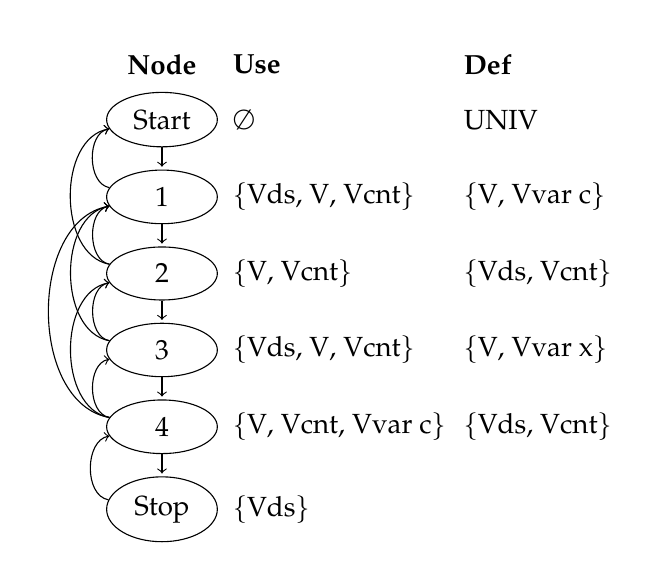
\begin{tikzpicture}
\matrix[
row sep=.8em,
    anchor=west,
    column 1/.append style={nodes={ellipse,draw,minimum width=4em,anchor=center}},
    ]{

	    \node[draw=none] {\textbf{Node}}; & \node {\textbf{Use}}; & \node {\textbf{Def}}; \\[-.8em]
		    \node (start) {Start}; & \node {$\emptyset$}; & \node {\isa{UNIV}}; \\
		    \node (1) {1}; & \node{\{\isa{Vds}, \isa{V\isasymbeta}, \isa{Vcnt}\}}; & \node{\{\isa{V\isasymbeta}, \isa{Vvar\ c}\}}; \\
		    \node (2) {2}; & \node{\{\isa{V\isasymbeta}, \isa{Vcnt}\}}; & \node{\{\isa{Vds}, \isa{Vcnt}\}}; \\
		    \node (3) {3}; & \node{\{\isa{Vds}, \isa{V\isasymbeta}, \isa{Vcnt}\}}; & \node{\{\isa{V\isasymbeta}, \isa{Vvar\ x}\}}; \\
		    \node (4) {4}; & \node{\{\isa{V\isasymbeta}, \isa{Vcnt}, \isa{Vvar\ c}\}}; & \node{\{\isa{Vds}, \isa{Vcnt}\}}; \\
		    \node (stop) {Stop}; & \node{\{\isa{Vds}\}}; \\
    };
\begin{scope}[shorten >=1pt]
\draw[->] (start) -- (1);
\draw[->] (1) -- (2);
\draw[->] (2) -- (3);
\draw[->] (3) -- (4);
\draw[->] (4) -- (stop);
\end{scope}

\begin{scope}[every to/.style={out=170, in=190, thick, shorten >=1pt}]
\draw[->] (stop) to (4);
\draw[->] (4) to (3);
\draw[->] (4) to (2);
\draw[->] (4) to (1);
\draw[->] (3) to (2);
\draw[->] (3) to (1);
\draw[->] (2) to (1);
\draw[->] (2) to (start);
\draw[->] (1) to (start);
\end{scope}
\end{tikzpicture}
\end{framed}
\caption{Naïve instantiation}
\label{fig:cfgsimp}
\end{figure}

\vref{fig:cfgsimp} contains the naive call graph without any of the modifications in the previous section. The program’s control flow is purely linear, denoted by down-pointing edges. Edges in the other direction denote dependencies between the nodes. The intermediate nodes which we added per edge to fulfill the framework’s requirements are not shown.

In this form, every node influences the final node and we do not obtain any useful information from the slicing analysis. In \vref{fig:cfgbetter}, we improved the instantiation by introducing special nodes to update the contour counter \isa{Vcnt} resp. the contour environment \isa{V\isasymbeta}. The figure contains only the dependency arrows relevant in the analysis of the stop node.

In this case, the analysis provides a useful result: The nodes 2 and 3, representing the useless call and the useless lambda, do not influence the Stop node. The corresponding extra nodes are still in the set of depending nodes. In that sense, they form the skeleton of the program flow and are never removed by slicing.


\begin{figure}
\begin{framed}
\centering
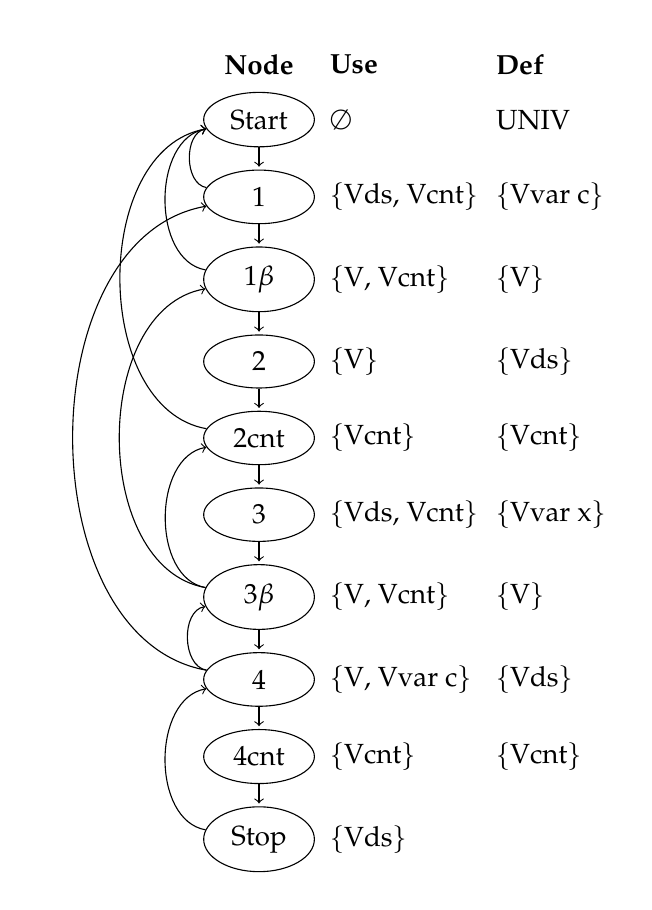
\begin{tikzpicture}
\matrix[
row sep=.8em,
    anchor=west,
    column 1/.append style={nodes={ellipse,draw,minimum width=4em,anchor=center}},
    ]{
	    \node[draw=none] {\textbf{Node}}; & \node {\textbf{Use}}; & \node {\textbf{Def}}; \\[-.8em]
		    \node (start) {Start}; & \node {$\emptyset$}; & \node {\isa{UNIV}}; \\
		    \node (1) {1}; & \node{\{\isa{Vds}, \isa{Vcnt}\}}; & \node{\{\isa{Vvar\ c}\}}; \\
		    \node (1b) {1$\beta$}; & \node{\{\isa{V\isasymbeta}, \isa{Vcnt}\}}; & \node{\{\isa{V\isasymbeta}\}}; \\
		    \node (2) {2}; & \node{\{\isa{V\isasymbeta}\}}; & \node{\{\isa{Vds}\}}; \\
		    \node (2b) {2cnt}; & \node{\{\isa{Vcnt}\}}; & \node{\{\isa{Vcnt}\}}; \\
		    \node (3) {3}; & \node{\{\isa{Vds}, \isa{Vcnt}\}}; & \node{\{\isa{Vvar\ x}\}}; \\
		    \node (3b) {3$\beta$}; & \node{\{\isa{V\isasymbeta}, \isa{Vcnt}\}}; & \node{\{\isa{V\isasymbeta}\}}; \\
		    \node (4) {4}; & \node{\{\isa{V\isasymbeta}, \isa{Vvar\ c}\}}; & \node{\{\isa{Vds}\}}; \\
		    \node (4b) {4cnt}; & \node{\{\isa{Vcnt}\}}; & \node{\{\isa{Vcnt}\}}; \\
		    \node (stop) {Stop}; & \node{\{\isa{Vds}\}}; \\
    };
\begin{scope}[shorten >=1pt]
\draw[->] (start) -- (1);
\draw[->] (1) -- (1b);
\draw[->] (1b) -- (2);
\draw[->] (2) -- (2b);
\draw[->] (2b) -- (3);
\draw[->] (3) -- (3b);
\draw[->] (3b) -- (4);
\draw[->] (4) -- (4b);
\draw[->] (4b) -- (stop);
\end{scope}

\begin{scope}[every to/.style={out=170, in=190, thick, shorten >=1pt}]
\draw[->] (stop) to (4);
\draw[->] (4) to (3b);
\draw[->] (4) to (1);
\draw[->] (3b) to (2b);
\draw[->] (3b) to (1b);
\draw[->] (2b) to (start);
\draw[->] (1)  to (start);
\draw[->] (1b)  to (start);
\end{scope}
\end{tikzpicture}
\end{framed}
\caption{Improved instantiation}
\label{fig:cfgbetter}
\end{figure}

\chapter{Conclusion}

\lettrine[lines=3]We have successfully formalized Shivers’ control flow analysis for functional programming languages and proven it correct. We employed the theorem prover Isabelle and chose the logic package \isa{HOLCF} to base our work on. This turned out to be the right choice for implementing denotational semantics. 

The formalization was, for the greatest part, straight forward. Where it was not, it was still possible to obtain the desired results, after some experimentation.

We outlined a possible connection to Daniel Wasserrab’s framework for formally verified slicing, discussed its problems and possible remedies. By a simple example, we showed that such a slicing analysis can be useful when applied to functional programs.

\appendix

{
\raggedright
% Space-Saving hack.
\renewcommand{\bibfont}{\setlength{\parskip}{-11pt}}
\bibliography{root}
}

% Erklärung unten drauf
\renewcommand{\cleardoublepage}{\clearpage}
\chapter*{Erklärung}

\lettrine H{iermit} erkläre ich, Joachim Breitner, dass ich die vorliegende Studienarbeit selb\-ständig
und ausschließlich unter Verwendung der angegebenen Quellen und Hilfsmittel verfasst
habe.
\vspace{20mm}
\begin{tabbing}
\rule{4cm}{.4pt}\hspace{1cm} \= \rule{7cm}{.4pt} \\
Ort, Datum \> Unterschrift
\end{tabbing}

\end{document}
